
\documentclass[12pt,notitlepage]{article}
%\usepackage{osa2}
%\usepackage{overcite}  %% PRODUCES SUPERSCRIPT REFERENCE CITATIONS
%\usepackage[comma,sort&compress,nonamebreak]{natbib}
%\bibpunct{[}{]}{,}{n}{}{,}
%\bibpunct{\textsuperscript{}}{\textsuperscript{}}{,}{s}{,}{,}
%\citestyle{nature}
\usepackage{epsfig,url}
\urlstyle{same}

\oddsidemargin      0in
\evensidemargin     0in
\setlength{\paperheight}{11in}%
\setlength{\paperwidth}{8.5in}%
\setlength{\textwidth}{\paperwidth}%
% subtract for the 1" top/bottom margins
\addtolength{\textwidth}{-2.0in}%
\setlength{\textheight}{\paperheight}%
\addtolength{\textheight}{-3.0in}%

\usepackage{setspace}
\usepackage{amsmath}
\usepackage{color}
\usepackage{caption} % so that I can have captions that dont wrap back under the caption index
\usepackage{hyperref}
\usepackage[T1]{fontenc}
\usepackage{lmodern}
\usepackage[ansinew]{inputenc}
\usepackage[all]{hypcap} % so that links to figures go to the figures and not the captions
\usepackage{subfig}   % subfigure
\captionsetup{format=hang,justification=raggedright}
\pagestyle{myheadings} \markboth{ Artifex Software Inc. www.artifex.com }{Artifex Software Inc. www.artifex.com}


\begin{document}

\begin{titlepage}

\begin{center}{\huge \bf Ghostscript 9.54 Color Management\\} \vspace{0.5in} {\Large Michael J.
Vrhel, Ph.D.\\} {\Large Artifex Software\\} {\Large 1305 Grant Avenue, Suite 200\\} {\Large Novato, CA 94945, USA\\}
{\Large www.artifex.com\\}
\end{center}
\vspace*{0.5in}
\begin{abstract}
This document provides information about the color architecture in Ghostscript 9.54. The document is suitable for users who wish to
obtain accurate color with their output device as well as for developers who wish to customize Ghostscript to achieve a higher
level of control and/or interface with a different color management module.
\end{abstract}
\begin{center}
\vspace*{0.25in}
Revision 1.66
\vspace*{0.25in}
\capstartfalse
\begin{figure}[h]
    \begin{center}
\includegraphics*[width=1.5in]{figures/ghostscriptR_stack_RGBclr_CS6.pdf}
    \end{center}
\end{figure}
\capstarttrue

\end{center}

\end{titlepage}

\renewcommand{\baselinestretch}{1.67}\normalsize
%\maketitle

\clearpage

\singlespace

\section{Introduction}

With release 9.0, the color architecture of Ghostscript was updated to primarily use the ICC\cite{ICC} format for its color management needs.  Prior to this release, Ghostscript's color architecture was based heavily upon PostScript\cite{PS} Color Management (PCM).  This is due to the fact that Ghostscript was designed prior to the ICC format and likely even before there was much thought about digital color management.  At that point in time, color management was very much an art with someone adjusting controls to achieve the proper output color.

Today, almost all print color management is performed using ICC profiles as opposed to PCM.  This fact along with the desire to create a faster, more flexible design was the motivation for the color architectural changes in release 9.0.  Since 9.0, several new features and capabilities  have been added. As of the 9.54 release, features of the color architecture include:
\begin{itemize}
\item Easy to interface different CMMs (Color Management Modules) with Ghostscript.
\item ALL color spaces are defined in terms of ICC profiles.
\item Linked transformations and internally generated profiles are cached.
\item Easily accessed manager for ICC profiles.
\item Easy to specify default profiles for source DeviceGray, DeviceRGB and DeviceCMYK color spaces.
\item Devices can readily communicate their ICC profiles and have their ICC profiles set.
\item Operates efficiently in a multithreaded environment.
\item Handles named colors (spots) with ICC named color profile or proprietary format.
\item ICC color management of Device-N colors or alternatively customizable spot color handing.
\item Includes object type (e.g. image, vector graphics, text), rendering intent and black point compensation into the computation of the linked transform.
\item Ability to override document embedded ICC profiles with Ghostscript's default ICC profiles.
\item Easy to specify unique {\bf source} ICC profiles to use with vector graphic, image and text objects.
\item Easy to specify unique {\bf destination} ICC profiles to use with vector graphic, image and text objects.
\item Easy to specify different rendering intents (perceptual, colorimetric, saturation, absolute colorimetric) for vector graphic, image and text objects.
\item Easy to specify different black point compensation settings for vector graphic, image and text objects.
\item Ability to make use of a PDF output intent ICC profile.
\item Ability to use an NCLR ICC output profile when rendering to a separation device.
\item Control to force gray source colors to black ink only when rendering to output devices that support black ink.
\item Ability to make use of device link ICC profiles for direct mapping of source colors to the device color space.
\item Ability to make use of device link ICC profiles for retargeting from SWOP/Fogra standard color space to a specific device color space.
\item Ability to monitor for the presence of color on individual pages, which is useful for certain print systems.
\item Ability to specify different default transparency blending color spaces.
\item Ability to specify a post rendering ICC profile for certain devices.
\item Ability to accurately simulate overprinting with spot colors regardless of the output device color capabilities.
\end{itemize}
The document is organized to first provide a high level overview of the architecture. This is followed by details of the various functions and structures, which include the information necessary to interface other color management modules to Ghostscript as well as how to interface specialized color handling operations.

\section{Overall Architecture and Typical Flow}

Figure \ref{fig:ICC_ARCH} provides a graphical overview of the various components that make up the architecture.  The primary components are:
\begin{itemize}
\item  The ICC manager, which maintains the various default profiles.
\item The link cache, which stores recently used linked transforms.
\item The profile cache, which stores internally generated ICC profiles created from PostScript CIE based color spaces and CalRGB, CalGray PDF color spaces.
\item The profiles contained in the root folder iccprofiles, which are used as default color spaces for the output device and for undefined source colors in the document.
\item The color management module (CMM), which is the engine that provides and performs the transformations (e.g. little CMS).
\item The profiles associated with the device, which include profiles dependent upon object type, a proofing profile and a device link profile.
\end{itemize}
In the typical flow, when a thread is ready to transform a buffer of data, it will request a linked transform from the link cache. When requesting a link, it is necessary to provide information to the CMM, which consists of a source color space, a destination color space, an object state (e.g. text, vector graphic, or image), black point compensation setting and a rendering type (e.g. perceptual, saturation, colorimetric).  The linked transform provides a mapping directly from the source color space to the destination color space. If a linked transform for these settings does not already exist in the link cache, a linked transform from the CMM will be obtained (assuming there is sufficient memory -- if there is not sufficient memory then the requesting thread will need to wait).  Depending upon the CMM, it is possible that the CMM may create a lazy linked object (i.e. create the real thing when it is asked to transform data).  At some point, a linked transform will be returned to the requesting thread.  The thread can then use this mapping to transform buffers of data through calls through an interface to the external CMM.  Once the thread has completed its use of the link transform, it will notify the link cache.  The link cache will then be able to release the link when it needs additional cache space due to other link requests.

\begin{figure}
    \begin{center}
  %  \leavevmode \epsfysize=3.0in
\includegraphics*[width=6.5in]{figures/architecture.pdf}
    \end{center}
   \caption{Graphical Overview of Ghostscript's Color Architecture}
    \label{fig:ICC_ARCH}
\end{figure}

\section{PDL Color Definitions and ICC Profiles}

To help reduce confusion, it is worthwhile to clarify terminology. In particular, the use of the terms process color and device color need to be defined in the context of ICC profiles. Both PDF\cite{PDF} and PostScript (PS) have a distinction between process colors and device colors.  In PS, there is
a conversion (e.g. via UCR/BG) from device colors to process colors.  In an ICC work flow, the colors are transformed directly from an input color space (often called the source space) to an output color space (often called the destination space).  The output color space defined by the device's ICC profile is a mapping to what PDF and PS define as the process color space of the device.  In other words, the ``device color space'' as defined by the device's ICC profile IS the process color space of PDF and PS.  The ICC profile of the device is a mapping from a CIE color space to the process color space AND from the process color space to a CIE color space.

To understand this better, it may help to understand the method by which a print based ICC profile is created.  To create an ICC profile for a device, a chart is printed using its process colors (e.g. CMYK).  This chart is measured using a colorimeter or a spectrophotometer.  This provides the forward mapping from process colors to CIELAB values.  The inverse mapping (from CIELAB to process colors) is obtained by inverting this table usually through a brute force search and extrapolation method.  These mappings are both packed into an ICC format, thereby defining mappings between the device ``process colors'' and the CIE color space.

\section{Usage}

There are a number of command line options available for color control.  These options are also available as device parameters and so can be set from Ghostscript's command prompt when Ghostscript is used in ``server-mode'' operation.

To define source colors that are not already colorimetrically defined in the source document, the following command line options can be invoked:\\

\textcolor{red}{-sDefaultGrayProfile = my\_gray\_profile.icc}\\

\textcolor{red}{-sDefaultRGBProfile = my\_rgb\_profile.icc}\\

\textcolor{red}{-sDefaultCMYKProfile = my\_cmyk\_profile.icc}\\

 \noindent In this case, for example, any Device Gray source colors will be interpreted as being defined by the ICC profile my\_gray\_profile.icc.  If these profiles are not set, default ICC profiles will be used to define undefined colors.  These default profiles are contained in the directory iccprofiles and are named default\_gray.icc, default\_rgb.icc and default\_cmyk.icc.  The profile default\_gray.icc is defined to provide output along the neutral axis with an sRGB linearization.  The profile default\_rgb.icc is the V2 sRGB ICC profile and the profile default\_cmyk.icc is a SWOP CMYK ICC profile.\\

It is possible to have Ghostscript use the above specified ICC profiles in place of ICC profiles embedded in the document.  This is achieved using\\

 \textcolor{red}{-dOverrideICC = true/false}\\

\noindent which, when set to true overrides any ICC profiles contained in the source document with the profiles specified by DefaultGrayProfile, DefaultRGBProfile, DefaultCMYKProfile. Note that if no profiles are specified for the default Device color spaces, then the system default profiles will be used for DeviceGray, DeviceRGB and DeviceCMYK source colors. For detailed override control in the specification of source colors see SourceObjectICC.\\

In addition to being able to define undefined source colors, it is possible to define the ICC profile for the output device using\\

\textcolor{red}{-sOutputICCProfile = my\_device\_profile.icc}\\

 \noindent Care should be taken to make sure that the number of components associated with the output device is the same as the number of components for the output device ICC profile (i.e. use an RGB profile for an RGB device).  If the destination device is CMYK + SPOT colorants, then it is possible to specify either a CMYK ICC profile or an N-Color ICC profile for the device.  If a CMYK profile is specified, then only the CMYK colorants will be color managed.  If an output profile is not specified, then the default CMYK profile is used as the output profile.\\

 If an N-Color (NCLR) ICC profile is specified for the output device (valid for tiffsep and psdcmyk devices), then it is possible to specify the name of the colorants in the profile.   This specification is done using\\

\textcolor{red}{-sICCOutputColors=``Cyan, Magenta, Yellow, Black, Orange, Violet''}\\

 \noindent where the colorants listed are shown as an example.  The list of the colorant names must be in the order that they exist in the profile.  Note that if a colorant name that is specified for the profile occurs also within the document (e.g. "Orange" above), then these colorants will be associated with the same separation. It is possible through a compile time option LIMIT\_TO\_ICC defined in gdevdevn.h to restrict the output colorants of the psdcmyk and tiffsep device to the colorants of the ICC profile or to allow additional spot colorants in the document to be created as different separations. If restricted, the other spot colorants will go through the alternate tint transform and then be mapped to the color space defined by the N-CLR profile.\\

 Note that if an NCLR profile is specified for the device and -sICCOutputColors is not specified, then the assumption will be that the first four colorants in the profile are cyan, magenta, yellow and black and the remaining spot colors will be named using the form ICC\_COLOR\_$i$ where $i$ is an index from 0 to the number of spot colors in the profile minus one.\\

A directory can be defined, which will be searched to find the above defined ICC profiles.  This makes it easier for users who have their profiles contained in a single directory and do not wish to append the full path name in the above command line options.  The directory is set using\\

\textcolor{red}{-sICCProfilesDir = c:/my\_icc\_profiles}\\

 \noindent Note that if the build of gs or other PDL languages is performed with COMPILE\_INITS=1, then the profiles contained in gs/iccprofiles will be placed in the ROM file system. If a directory is specified on the command line using -sICCProfilesDir=, that directory is searched before the iccprofiles/ directory of the ROM file system is searched.

Named color support for separation color spaces is specified through the command line option\\

\textcolor{red}{-sNamedProfile = c:/my\_namedcolor\_structure}\\

 \noindent While the ICC specification does define a named color format, the above structure can in practice be much more general for those who have complex handling requirements of separation color spaces. For example, some developers wish to use their own proprietary-based format for spot color management. This command option is for developer use when an implementation for named color management is designed for the function {\bf gsicc\_transform\_named\_color} located in gsicc\_cache.c . An example implementation is currently contained in the code [see comments above {\bf gsicc\_transform\_named\_color} in gsicc\_cache.c]. For the general user, this command option should really not be used.\\

The above option deals with the handling of single spot (Separation) colors as well as with DeviceN colors.  An example of its use for DeviceN and Separation colors is given in gs/toolbin/color/named\_color, where you will want to use the command line option -sNamedProfile=named\_color\_table.txt.\\

 It is also possible to specify ICC profiles for managing DeviceN source colors. This is done using the command line option\\

\textcolor{red}{-sDeviceNProfile = c:/my\_devicen\_profile.icc}\\

 \noindent Note that neither PS nor PDF provide in-document ICC profile definitions for DeviceN color spaces. With this interface it is possible to provide this definition. The colorants tag order in the ICC profile defines the lay-down order of the inks associated with the profile. A windows-based tool for creating these source profiles is contained in gs/toolbin/color/icc\_creator.  If non-ICC based color management of DeviceN source colors is desired by a developer, it is possible to use the same methods used for the handling of individual spot colors as described above.\\

The command line option\\

\textcolor{red}{-sProofProfile = my\_proof\_profile.icc}\\

\noindent enables the specification of a proofing profile, which will make the color management system link multiple profiles together to emulate the device defined by the proofing profile.  See Section \ref{sec:proof_link} for details on this option.\\

The command line option\\

\textcolor{red}{-sDeviceLinkProfile = my\_link\_profile.icc}\\

 \noindent makes it possible to include a device link profile in the color transformations.  This is useful for work flows where one wants to map colors first to a standard color space such as SWOP or Fogra CMYK, but it is desired to redirect this output to other CMYK devices. See Section \ref{sec:proof_link} for details on this option.\\

It is possible for a document to specify the rendering intent to be used when performing a color transformation.  Ghostscript is set up to handle four rendering intents with the nomenclature of Perceptual, Colorimetric, Saturation, and Absolute Colorimetric, which matches the terminology used by the ICC format.  By default, per the specification, the rendering intent is Relative Colorimetric for PDF and PS documents.  In many cases, it may be desired to ignore the source settings for rendering intent.  This is achieved through the use of\\

\textcolor{red}{-dRenderIntent = intent}\\

\noindent which sets the rendering intent that should be used with the profile specified above by -sOutputICCProfile. The options for intent are 0, 1, 2 and 3, which correspond to the ICC intents of Perceptual, Colorimetric, Saturation, and Absolute Colorimetric.\\

Similarly, it is possible to turn off or on black point compensation for the color managed objects in the document.  Black point compensation is a mapping performed near the black point that ensures that the luminance black in a source color space is mapped to the luminance black in a destination color space with adjustments to ensure a smooth transition for near black colors.  The mapping is similar to the mapping performed at the white point between devices. With black point compensation enabled, potential loss of detail in the shadows is reduced.   By default, Ghostscript has black point compensation  enabled.  However, note that the PDF 2.0 specification adds a black point compensation member to the extended graphic state.  As such, it is possible that the document could turn off black point compensation.   If this is not desired, it is possible to force black point compensation to a particular state using\\

\textcolor{red}{-dBlackPtComp = 0 / 1}\\

\noindent where 0 implies compensation is off and 1 implies that compensation if on.  Integer values were used instead of boolean for this command to enable easy expansion of the option to different types of black point compensation methods.\\

It is also possible to make use of the special black preserving controls that exist in littleCMS.  The command line option\\

\textcolor{red}{-dKPreserve = 0 / 1 / 2}\\

\noindent specifies if black preservation should be used when mapping from CMYK to CMYK.   When using littleCMS as the CMM, the code 0
corresponds to no preservation, 1 corresponds to the PRESERVE\_K\_ONLY approach described in the littleCMS documentation and 2 corresponds to the PRESERVE\_K\_PLANE approach.
See the lcms users manual for details on what these options mean.\\

Ghostscript currently provides overprint simulation for spot colorants when rendering to the separation devices psdcmyk and tiffsep.  These devices maintain all the spot color planes and merge these together to provide a simulated preview of what would be printed.   Work is currently under development to provide overprint simulation to the other devices through the use of an intermediate compositing device.\\

There are three additional special color handling options that may be of interest to some users.  One is\\

\textcolor{red}{-dDeviceGrayToK = true/false}\\

\noindent By default, Ghostscript will map DeviceGray color spaces to pure K when the output device is CMYK based. The gray\_to\_k.icc profile in ./profiles is used to achieve this mapping of source gray to the colorant K.  The mapping of gray to K may not always be desired. In particular, it may be desired to map from the gray ICC profile specified by -sDefaultGrayProfile to the output device profile. To achieve this, one should specify -dDeviceGrayToK=false.\\

In certain cases, it may be desired to {\bf not} perform ICC color management on DeviceGray, DeviceRGB and DeviceCMYK source colors.  This can occur in particular if one is attempting to create an ICC profile for a target device and needed to print pure colorants.  In this case, one may want instead to use the traditional Postscript 255 minus operations to convert between RGB and CMYK with black generation and undercolor removal mappings.  To achieve these types of color mappings use the following command set to true\\

\textcolor{red}{-dUseFastColor = true/false}\\

\subsection{Output Intents and Post Rendering Color Management}
\label{sec:Transparency}
PDF documents can contain target ICC profiles to which the document is designed to be rendered.  These are called output intents within the PDF specification.   It is possible to make use of these profiles with the use of the command line option\\

\textcolor{red}{-dUsePDFX3Profile = int}\\

If this option is included in the command line, source device color values (e.g DeviceCMYK, DeviceRGB, or DeviceGray) that match the color model of the output intent will be interpreted to be in the output intent color space. In addition, if the output device color model matches the output intent color model, then the destination ICC profile will be the output intent ICC profile. If there is a mismatch between the device color model and the output intent, the output intent profile will be used as a proofing profile, since that is the intended rendering. Note that a PDF document can have multiple rendering intents per the PDF specification. As such, with the option -dUsePDFX3Profile the first output intent encountered will be used. It is possible to specify a particular output intent where int is an integer (a value of 0 is the same as not specifying a number). Probing of the output intents for a particular file is possible using extractICCprofiles.ps in ./gs/toolbin. Finally, note that the ICC profile member entry is an option in the output intent dictionary. It is possible for the output intent dictionary to specify a registry and a standard profile (e.g. Fogra39) instead of providing a profile. Ghostscript will not make use of these output intents. Instead, if desired, these standard profiles should be used with the commands specified above (e.g. -sOutputICCProfile).  Note that it is possible that a rendering intent can be an NCLR profile.  In this case, it is necessary to ensure that the device can handle such a profile (e.g. the psdcmyk and tiffsep devices).  In addition, the colorant names should be specified using -sICCOutputColors.

When using the output intent, but going to an output color space that is different than the actual intent, it may be desirable to apply an ICC transformation on the rendered output buffer.  For example, it may be necessary to render to the output intent ICC profile color space to ensure proper color blending, overprinting and that other complex operations occur as intended by the document author.   Once the document is rendered, we would want to transform to the color space defined for our actual output device.   The tiffscaled devices as well as the tiffsep device allow the specification of a post render ICC profile to achieve this.   The command line option is made using\\

\textcolor{red}{-sPostRenderProfile = my\_postrender\_profile.icc}\\

Note that this allows for the cases where the output intent color space of the document is CMYK based while the output device is RGB based.  In such a situation we would use a PostRenderProfile that was RGB based.

\subsection{Transparency and Color Management}
\label{sec:Transparency}
Transparency blending in PDF can be dependent upon the color space in which the blending takes place.  In certain source files, the color space for which the blending is to occur is not specified.  Per the specification, when this occurs, the color space of the target device should be used.   For consistent output across different device types this is not always desirable.   For this reason, Ghostscript provides the capability to specify the desired default blending color space through the command line option\\

\textcolor{red}{-sBlendColorProfile = my\_blend\_profile.icc}\\

\noindent When this option is used, if a source file has transparency blending the blending result should not depend upon the output device color model.

Ghostscript has the capability to maintain object type information even through transparency blending.  This is achieved through the use of a special tag plane during the blending of the objects.  When the final blending of the objects occurs this tag information is available.  Mixed objects will be indicated as such (e.g text blended with image).  A device can have a specialized put\_image operation that can handle the pixel level color management operation and apply the desired color mapping for different blend cases.  The bittagrgb device in Ghostscript provides a demonstration of the use of the tag information.

\subsection{Proof and Device-Link Profiles}
\label{sec:proof_link}

As shown in Figure \ref{fig:ICC_ARCH}, the proofing profile and the device link profile are associated with the device.  If these profiles have been specified using the options
-sProofProfile = my\_proof\_profile.icc and -sDeviceLinkProfile = my\_link\_profile.icc, then when the graphics library maps a source color defined by the ICC profile source.icc to the device color values, a transformation is computed by the CMM that consists of the steps shown in Figure \ref{fig:proof_link}. In this Figure, Device ICC Profile is the ICC profile specified for the actual device (this can be specified using -sOutputICCProfile).  In practice, the CMM will create a single mapping that performs the transformation of the multiple mappings shown in Figure \ref{fig:proof_link}.  If we specify a proofing profile, then our output should provide a proof of how the output would appear if it had been displayed or printed on the proofing device defined by the proofing profile.  The device link profile is useful for cases where one may have a work flow that consists of always rendering to a common CMYK space such as Fogra 39 followed by a mapping with a specialized device link profile.  In this case, the profile specified by -sOutputICCProfile would be the profile for the common CMYK space.

\begin{figure}
    \begin{center}
  %  \leavevmode \epsfysize=3.0in
\includegraphics*[width=7in]{figures/proof_link.pdf}
    \end{center}
   \caption{Flow of data through source, proof, destination and device link ICC profiles}
   \label{fig:proof_link}
\end{figure}

Note that if -sSourceObjectICC is used to specify device link ICC profiles to map from source color spaces to device colors, then it is not possible to use either the device profile or the proofing profile for these objects.  However, a device link profile that is associated with the target device will be merged with the device link profile specified for the source object.

\subsection{Object dependent color management}

It is often desired to perform unique mappings based upon object types.  For example, one may want to perform one color transformation on text colors to ensure a black text and a different transformation on image colors to ensure perceptually pleasing images and yet another transformation on graphics to create saturated colors.   To achieve this, Ghostscript provides an unprecedented amount of color control based upon object type.

The following commands, enable one to specify unique {\bf output} ICC profiles, rendering intents, black point compensation and black preserving methods for text, vector graphic, and image objects.  As shown in Figure \ref{fig:ICC_ARCH}, these profiles are stored in the device structure.  Specifically, the command options are:\\

\textcolor{red}{-sVectorICCProfile = filename}\\

\noindent Sets the ICC profile that will be associated with the output device for vector graphics (e.g. solid color Fill, Stroke operations). This option can be used to obtain more saturated colors for graphics.  Care should be taken to ensure that the number of colorants associated with the device is the same as the profile. \\

\textcolor{red}{-dVectorIntent = intent}\\

\noindent Sets the rendering intent that should be used with the profile specified above by -sVectorICCProfile. The options are the same as specified for -dRenderIntent.\\

\textcolor{red}{-dVectorBlackPt = 0 / 1}\\

\noindent Sets the black point compensation setting that should be used with the profile specified above by -sVectorICCProfile.\\

\textcolor{red}{-dVectorKPreserve = 0 / 1 / 2}\\

\noindent specifies the black preserving method that should be used from mapping CMYK to CMYK for vector graphic objects.   The
options are the same as specified for -dKPreserve.\\

\textcolor{red}{-sImageICCProfile = filename}\\

\noindent Sets the ICC profile that will be associated with the output device for images.  This can be used to obtain perceptually pleasing images.
Care should be taken to ensure that the number of colorants associated with the device is the same as the profile. \\

\textcolor{red}{-dImageIntent = intent}\\

\noindent Sets the rendering intent that should be used with the profile specified above by -sImageICCProfile. The options are the same as specified for -dRenderIntent. \\

\textcolor{red}{-dImageBlackPt = 0 / 1}\\

\noindent Sets the black point compensation setting that should be used with the profile specified above by -sImageICCProfile.\\

\textcolor{red}{-dImageKPreserve = 0 / 1 / 2}\\

\noindent specifies the black preserving method that should be used from mapping CMYK to CMYK for image objects.   The
options are the same as specified for -dKPreserve.\\

\textcolor{red}{-sTextICCProfile = filename}\\

\noindent Sets the ICC profile that will be associated with the output device for text.  This can be used ensure K only text at the output. Care should be taken to ensure that the number of colorants associated with the device is the same as the profile.\\

\textcolor{red}{-dTextIntent = intent}\\

\noindent Sets the rendering intent that should be used with the profile specified above by -sTextICCProfile. The options are the same as specified for -dRenderIntent. \\

\textcolor{red}{-dTextBlackPt = 0 / 1}\\

\noindent Sets the black point compensation setting that should be used with the profile specified above by -sTextICCProfile.\\

\textcolor{red}{-dTextKPreserve = 0 / 1 / 2}\\

\noindent specifies the black preserving method that should be used from mapping CMYK to CMYK for text objects.   The
options are the same as specified for -dKPreserve.\\

In addition to being able to have the output ICC profile dependent upon object type, it is possible to have the {\bf source} ICC profile and rendering intents be dependent upon object types for GRAY, RGB and CMYK objects.  Because this requires the specification of many new parameters and is only used in specialized situations, the specification is made through a single text file.  The text file is specified to Ghostscript using\\

\textcolor{red}{-sSourceObjectICC = filename}\\

This option provides an extreme level of override control to specify the source color spaces, rendering intents and black point compensation to use with vector graphics, images and text for source objects. The specification is made through a file that contains on a line, a key name to specify the object type (e.g. Image\_CMYK) followed by an ICC profile file name, a rendering intent number (0 for perceptual, 1 for colorimetric, 2 for saturation, 3 for absolute colorimetric), a black point compensation value (0 or 1), a boolean to indicate if source ICC profiles should be overridden, and a value for the CMYK objects to indicate if any type of black preservation should be used when going from CMYK to CMYK transformations. An example file is given in ./gs/toolbin/color/src\_color/objsrc\_profiles\_example.txt. Profiles to demonstrate this method of specification are also included in this folder. Note that if objects are colorimetrically specified through this mechanism, other operations like -sImageIntent, -dOverrideICC, have no affect.\\

The example file mentioned above contains the following tab delimited lines\\

\begin{tabular}{llllll}
Vector\_CMYK & cmyk\_src\_cyan.icc	& 0 & 1 & 0 & 0 \\
Image\_CMYK	& cmyk\_src\_magenta.icc &	0 & 1 & 0 & 0  \\
Text\_CMYK	& cmyk\_src\_yellow.icc	 & 0 & 1 & 0 & 0  \\
Vector\_RGB &	rgb\_source\_red.icc	& 0 & 1 & 0 & \\
Image\_RGB &	rgb\_source\_green.icc	& 0 & 1 & 0 & \\
Text\_RGB & rgb\_source\_blue.icc & 0 & 1 & 0 & \\
\end{tabular}\\

\noindent where the first item in the line is the key word, the second item in the line is the file name of the {\bf source} ICC profile to use for that object type, the third item specifies the rendering intent, the fourth item specifies the black point compensation setting, the fifth term indicates if source ICC profiles should be overridden, and the sixth term which should only be there for CMYK source objects indicates if any type of black preservation should be performed if we are going to a CMYK color space.  Note that not all types need to be specified.  It is possible to have only a single type specified in the file (e.g. Image\_CMYK).  The other items would render in a normal default fashion in this case.  Note that it is necessary to include all the possible options in each line.    That is, ``Vector\_CMYK  cmyk\_src\_cyan.icc 0'' is not a valid line but must include settings for the next three values as given above for Vector\_CMYK.  In addition to CMYK and RGB types given above, the user can also specify Vector\_GRAY, Image\_GRAY and Text\_GRAY objects.

In addition, it is possible to have unique color management methods for these object types through two special names which are ``None'' and ``Replace''.   For example, if our file contained the following two lines\\

\begin{tabular}{ll}
Vector\_CMYK & None \\
Text\_CMYK	& Replace  \\
\end{tabular}\\

\noindent then vector graphic CMYK source objects will not be color managed but instead will go through the standard Postscript mapping methods (e.g. 255-X).   CMYK text objects will go through the color replacement color management route which is provided for those developers who wish to provide direct output replacement colors for a given incoming source color.  This is currently implemented in the function gsicc\_rcm\_transform\_general, which is in the file gsicc\_replacecm.c.  The current implementation computes the color negative of the source color as a demonstration.  Note that the replaced color should be in the device's color space.   The entire contents of the file, gsicc\_replacecm.c are provided as an example for developers.

In addition, one can specify a device link ICC profile to use with a particular source object type when mapping to the destination color space.  This is done by simply using a notation such as\\

\begin{tabular}{llllll}
Vector\_RGB &	linkRGBtoCMYK.icc	& 0 & 1 & 0 & \\
\end{tabular}\\

\noindent in the -sSourceObjectICC file, where linkRGBtoCMYK.icc is the device link ICC profile file name.  Note that the rendering intent etc are still specified but their effect is dependent upon the CMM that is hooked in with Ghostscript.  With the current use of lcms, these values have no effect with device link profiles.   Note also that if the device ICC profile is an NCLR profile, it is possible that the device link profiles specified in the -sSourceObjectICC file can have a destination color space that is either CMYK or NCLR.

For those interested in this level of control, it is recommended to execute a number of examples.
In the first example, copy the files in ./gs/toolbin/color/src\_color/ to ./iccprofiles and render the file ./examples/text\_graph\_image\_cmyk\_rgb.pdf with the option -sSourceObjectICC = objsrc\_profiles\_example.txt to an RGB device (e.g. tiff24nc).  Note, to ensure that Ghostscript can find all the files and to avoid having to do a full rebuild to create the ROM file system, you may want to specify the icc directory using\\
 -sICCProfilesDir=``your\_full\_path\_to\_iccprofiles/", which provides the full path to ./iccprofiles/.   Windows users should be sure to use the forward slash delimiter due to the special interpretation of ``\textbackslash'' by the Microsoft C startup code.

\begin{figure}
    \begin{center}
  %  \leavevmode \epsfysize=3.0in
\includegraphics*[width=2.5in]{figures/text_graph_image_cmyk_rgb.pdf}
    \end{center}
   \caption{Example file with mixed content. The file includes RGB and CMYK text, vector graphics, and images}
    \label{fig:normal}
\end{figure}

\begin{figure}
  \subfloat[Source profiles vary with object type]{\label{fig:source_icc}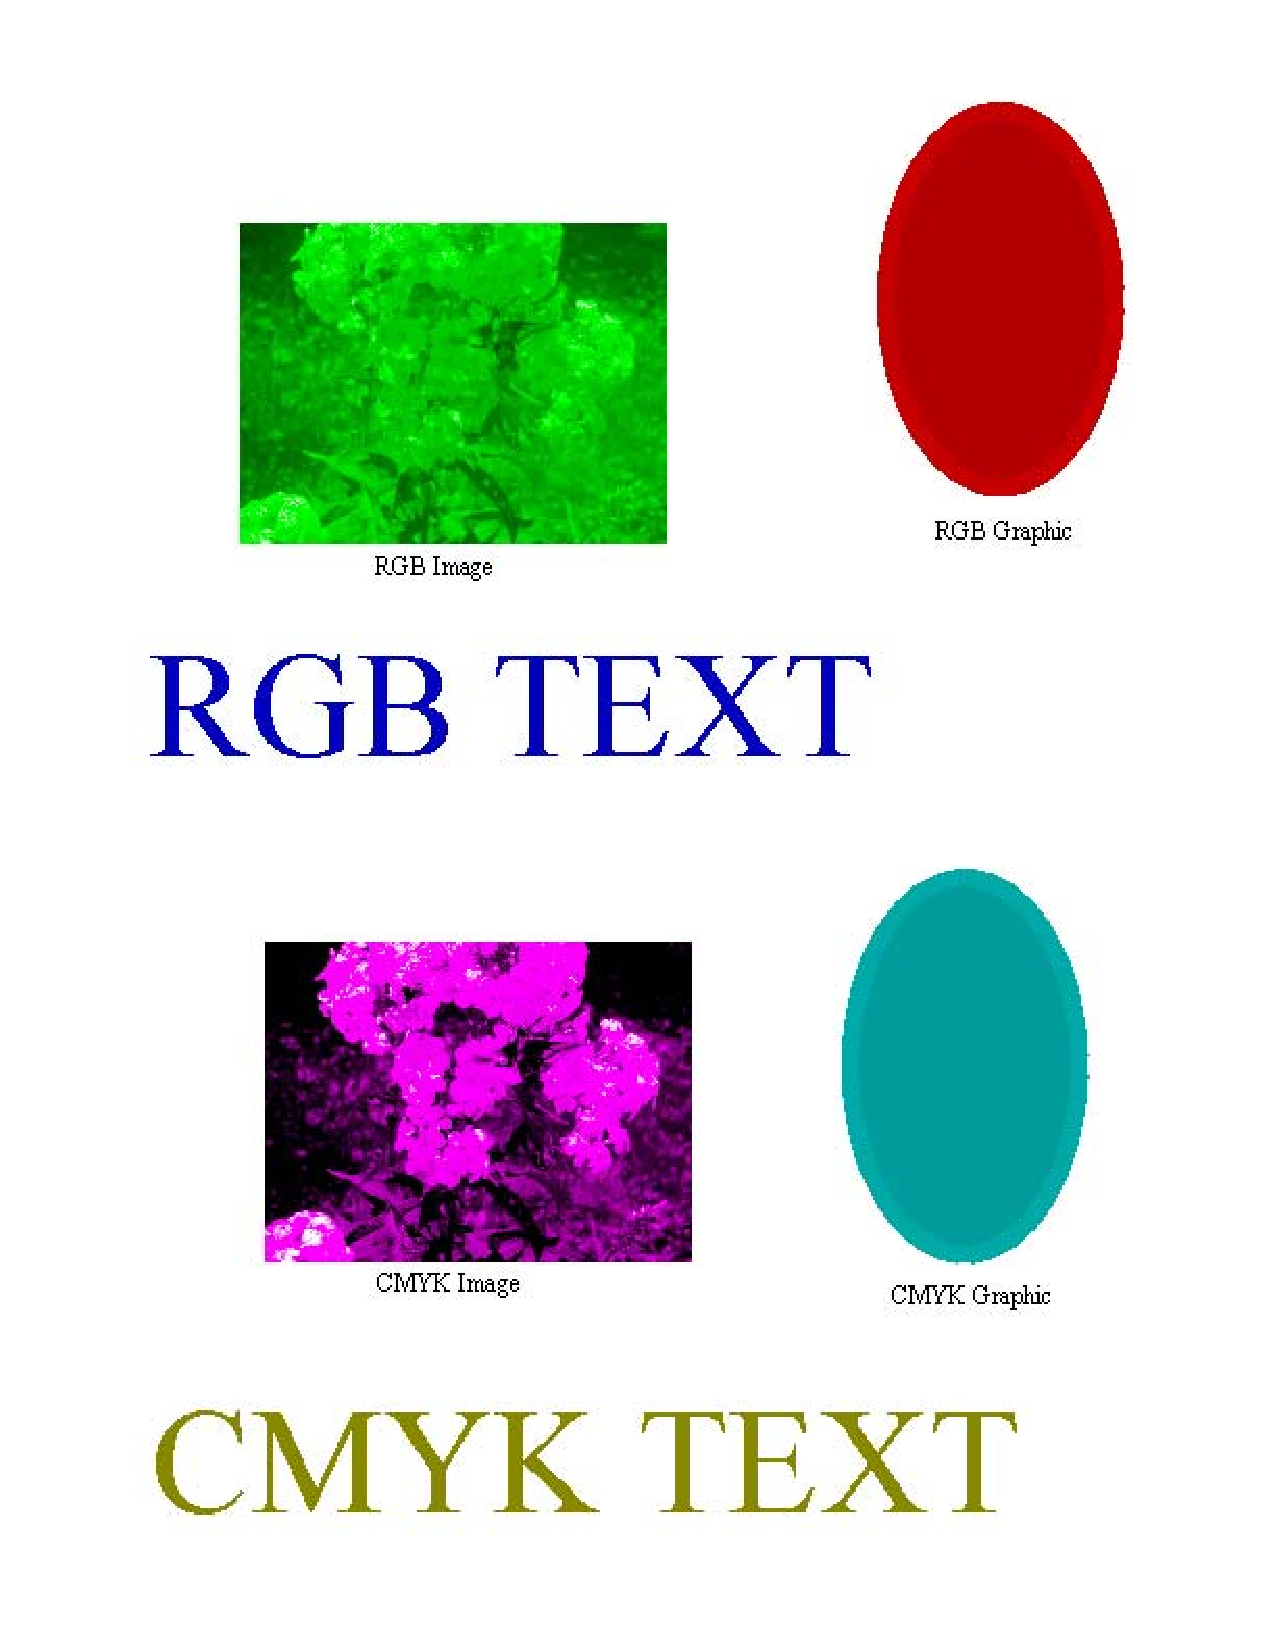
\includegraphics[width=0.5\textwidth]{figures/source_profile.pdf}}
  \subfloat[Rendering intents vary with CMYK source object type]{\label{fig:source_ri}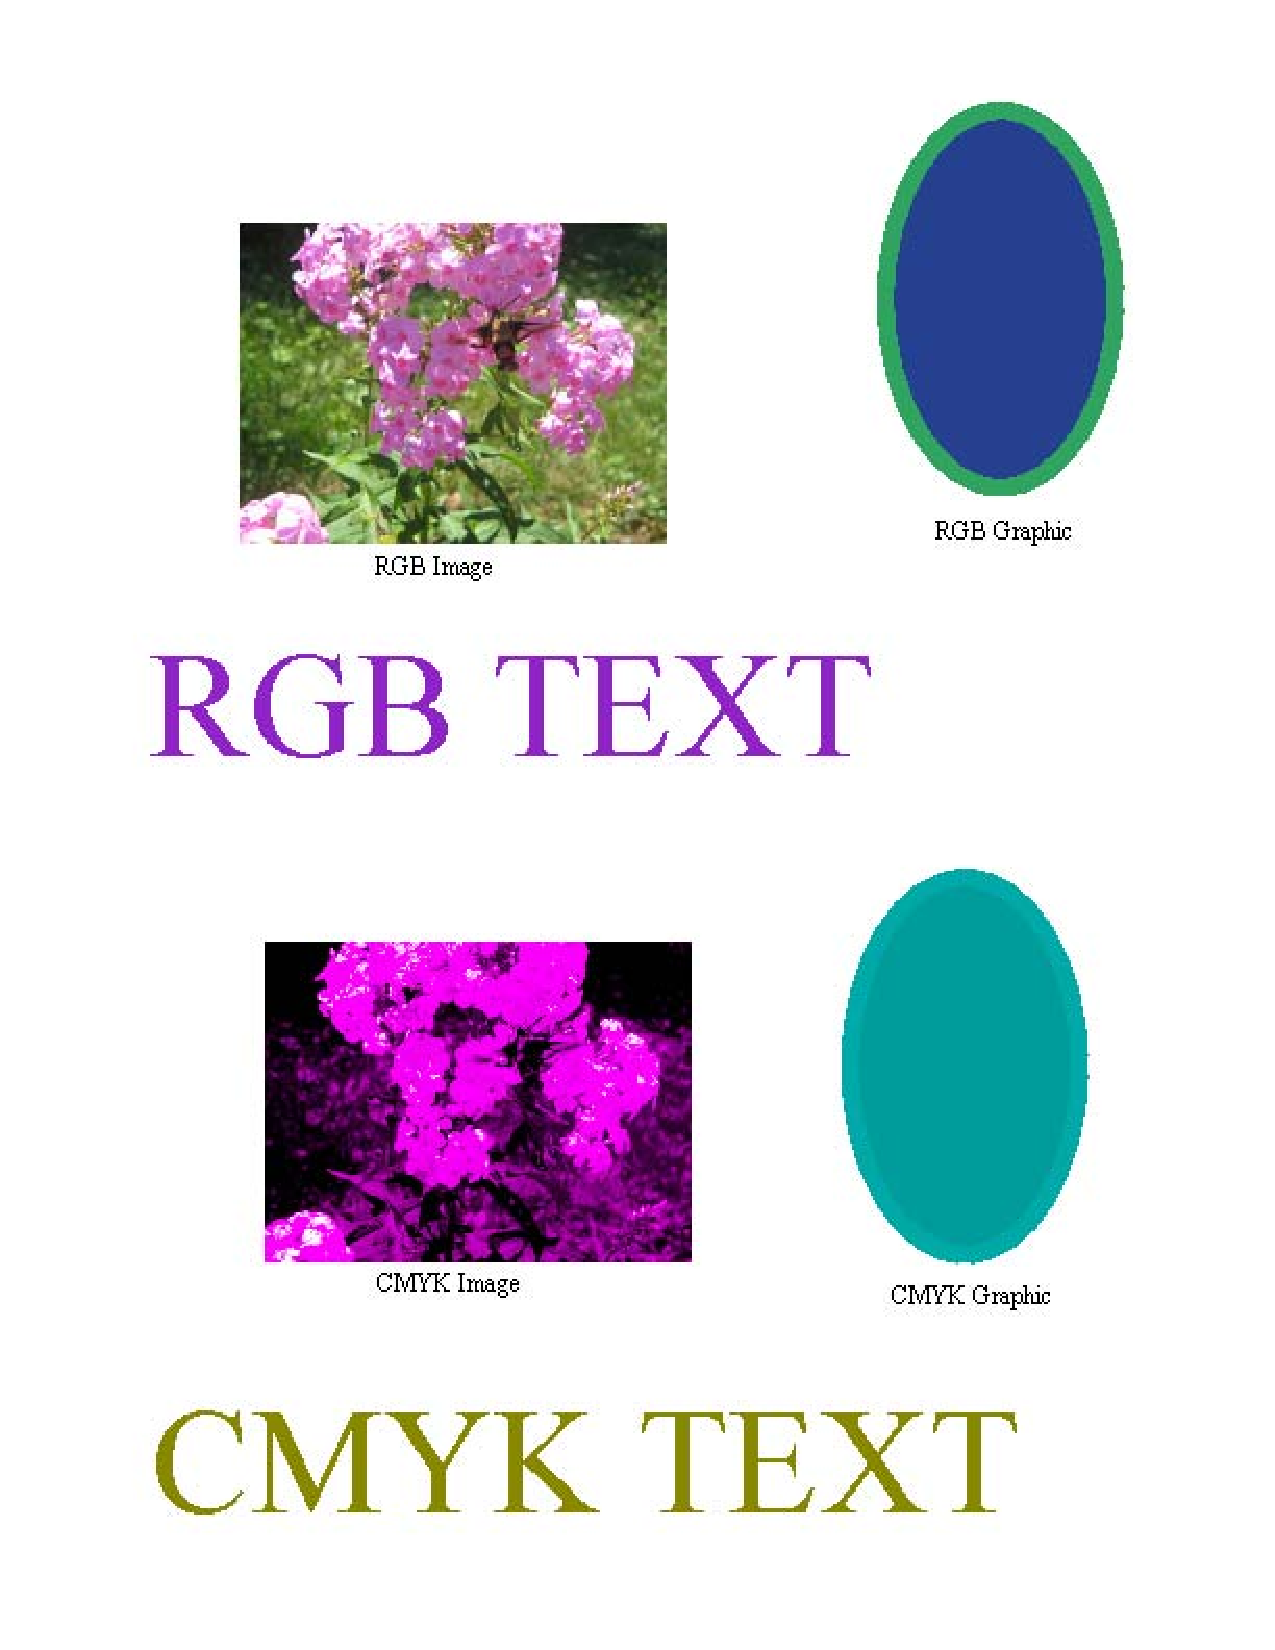
\includegraphics[width=0.5\textwidth]{figures/source_intent.pdf}}
    \caption{Examples of object based color transformations for the file from Figure \ref{fig:normal} by specifying {\bf source} profiles and/or rendering intents}
\end{figure}

\begin{figure}
  \subfloat[Destination profiles vary with object type]{\label{fig:des_icc}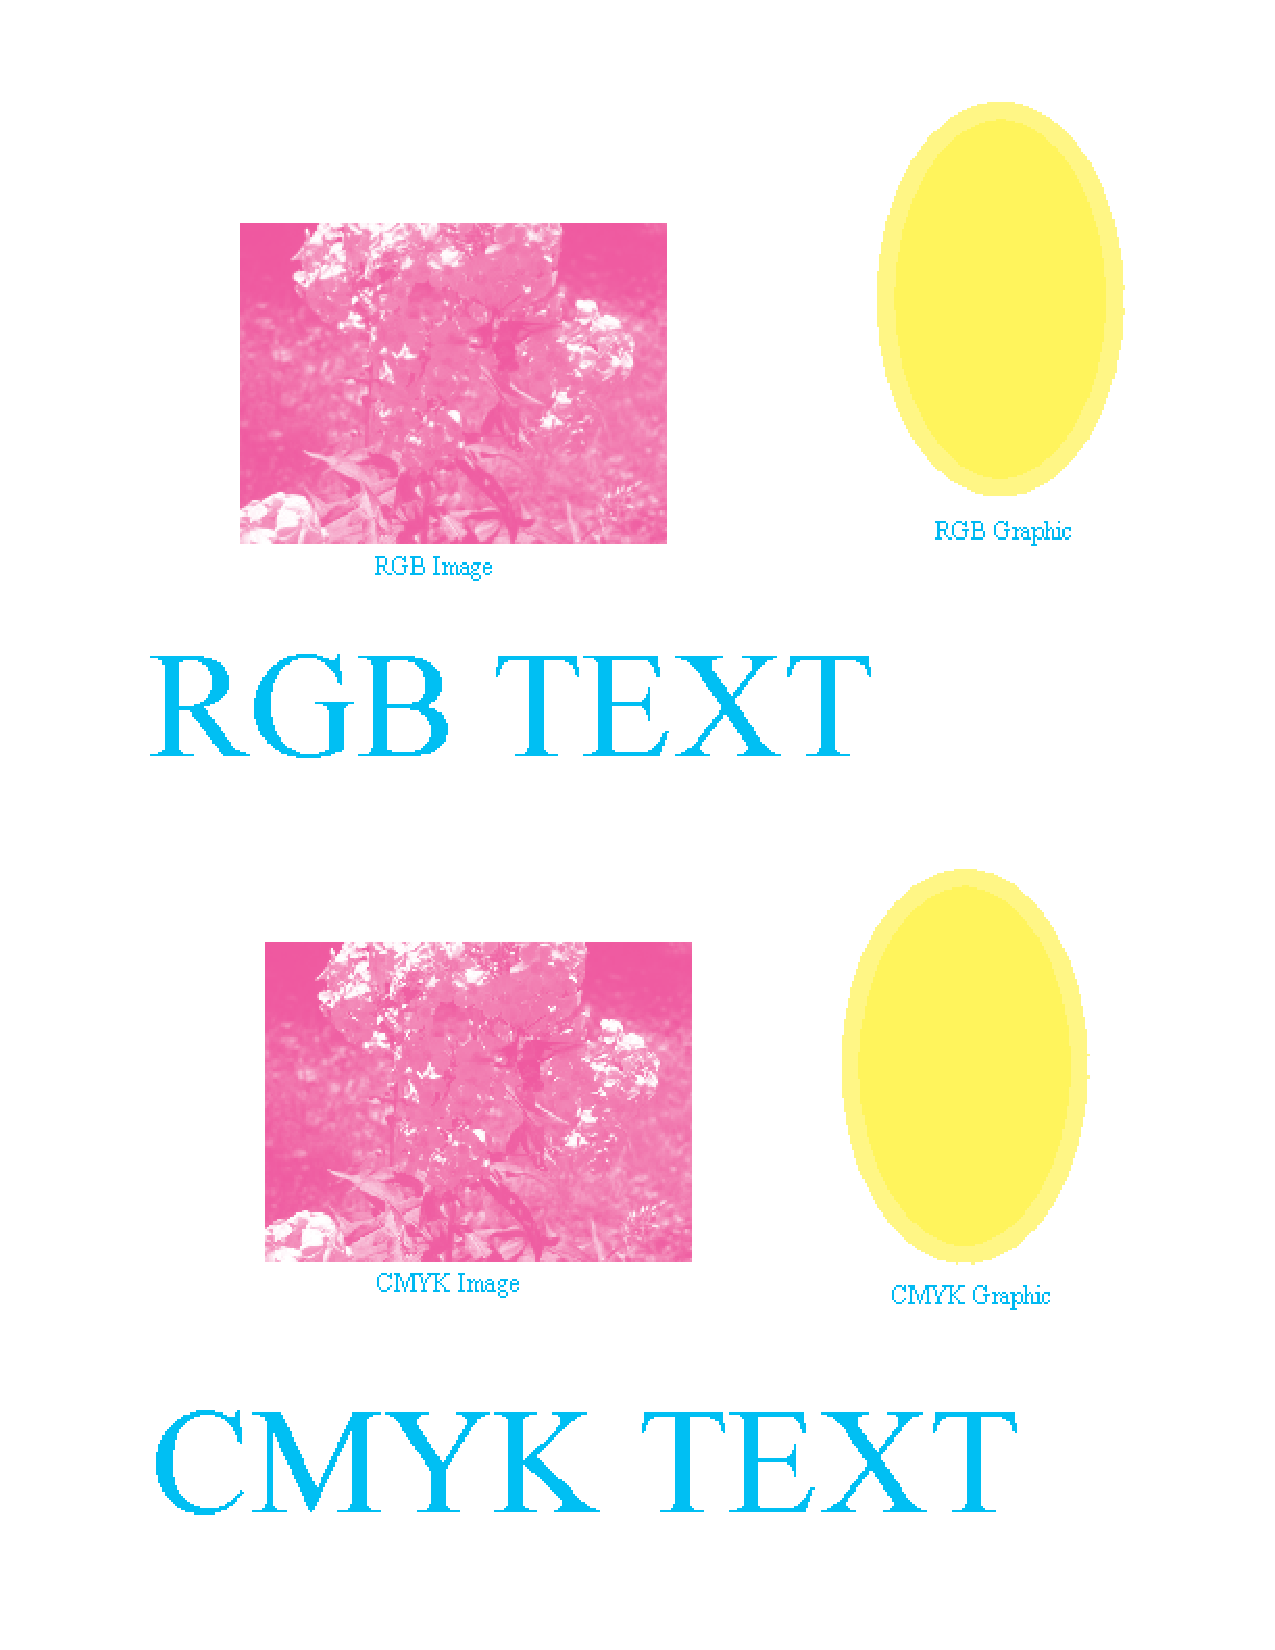
\includegraphics[width=0.5\textwidth]{figures/destination_profile.pdf}}
  \subfloat[Destination intents vary with object type]{\label{fig:des_ri}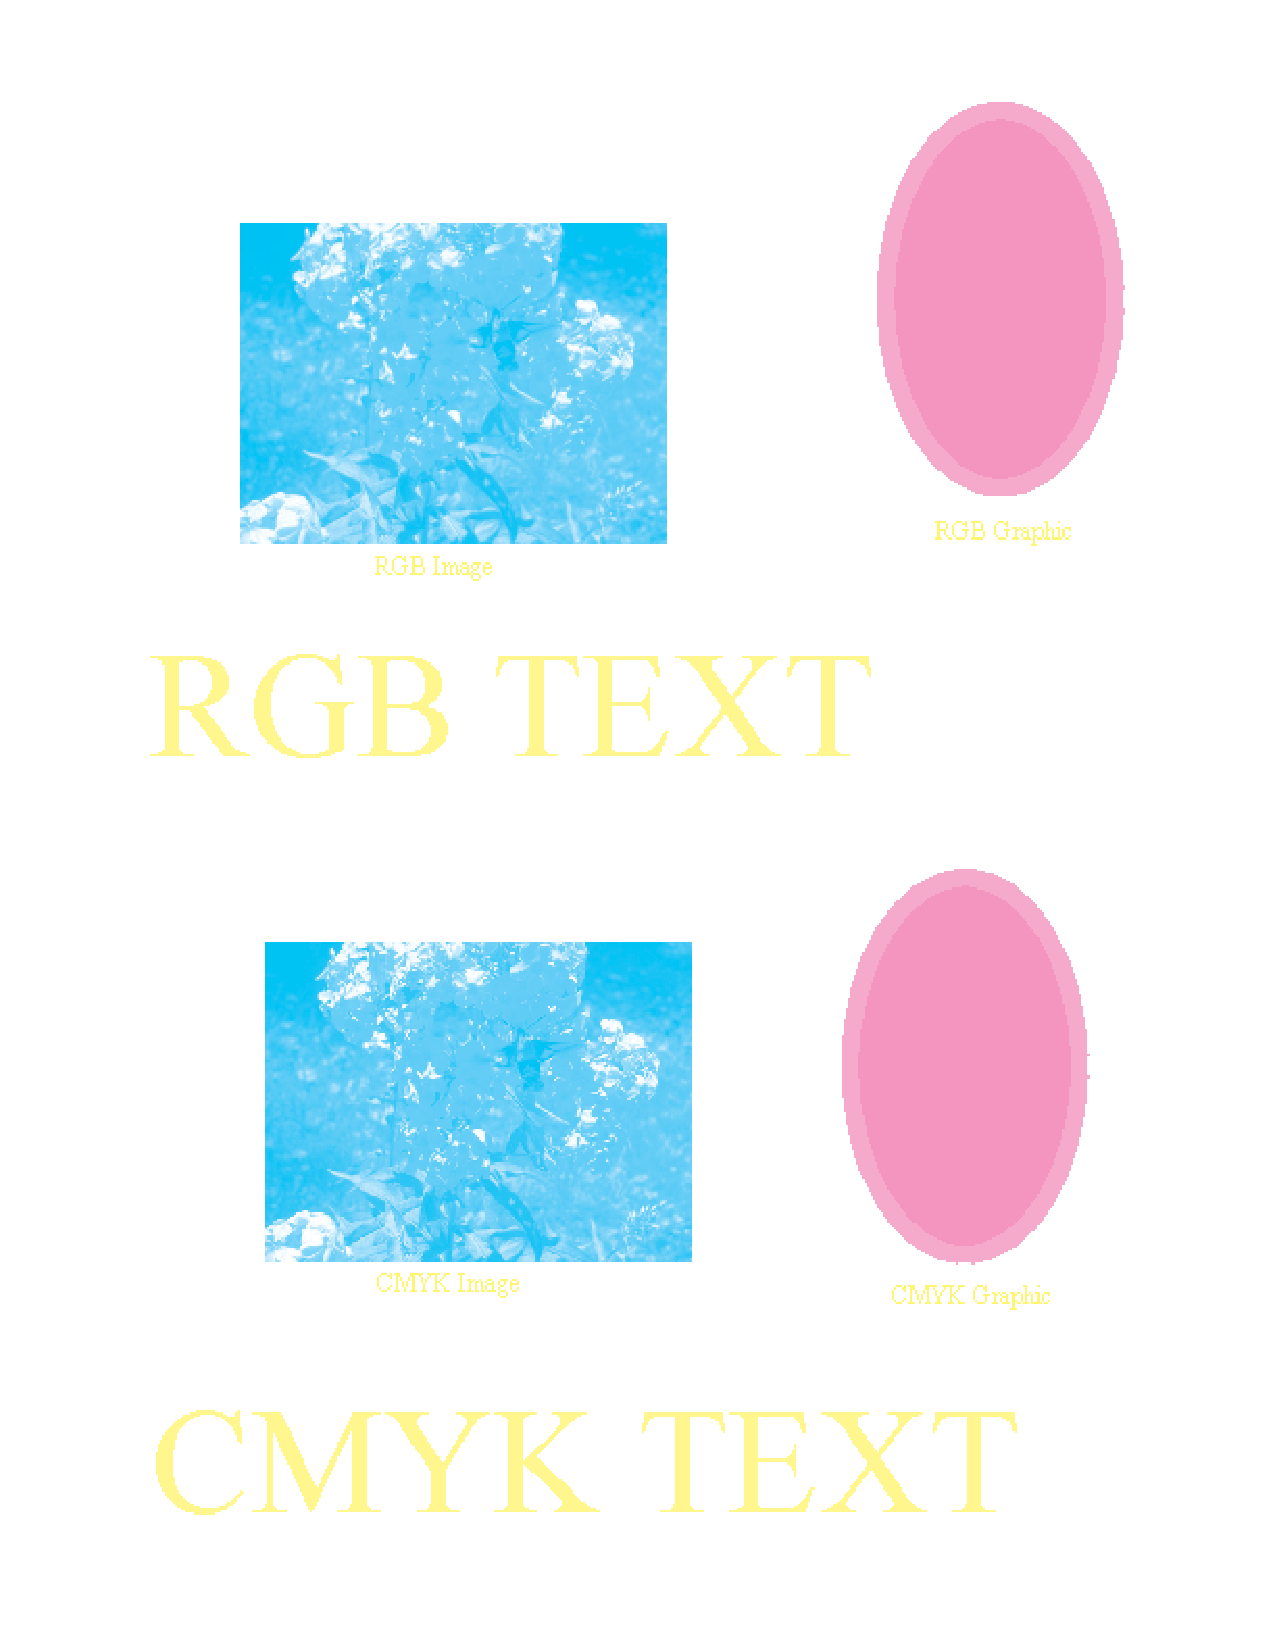
\includegraphics[width=0.5\textwidth]{figures/des_profile_intent.pdf}}
    \caption{Examples of object based color transformations for the file from Figure \ref{fig:normal} by specifying {\bf destination} profiles and/or intents}
  \label{fig:object_based_color}
\end{figure}

Figure \ref{fig:normal} displays the source file text\_graph\_image\_cmyk\_rgb.pdf rendered with default settings and Figure \ref{fig:source_icc} displays the result when rendered using  -sSourceObjectICC = objsrc\_profiles\_example.txt.   The profiles specified in objsrc\_profiles\_example.txt are designed to render object types to the color specified in their name when used as a source profile.  In this case, RGB vector graphics, images and text are rendered red, green and blue respectively and CMYK  vector graphics, images and text are rendered cyan, magenta and yellow respectively.\\

Modifying the contents of the objsrc\_profiles\_example.txt file to\\

\begin{tabular}{llllll}
Vector\_CMYK & cmyk\_src\_renderintent.icc	& 0 & 1 & 0 & 0\\
Image\_CMYK	& cmyk\_src\_renderintent.icc	& 1 & 1 & 0 & 0 \\
Text\_CMYK	& cmyk\_src\_renderintent.icc	& 2 & 1 & 0 & 0 \\
\end{tabular}\\

\noindent and rendering the file ./examples/text\_graph\_image\_cmyk\_rgb.pdf to an RGB device, one obtains the output shown in Figure \ref{fig:source_ri}.  In this case, we demonstrated the control of rendering intent based upon object type.  The profile cmyk\_src\_renderintent.icc is designed to create significantly different colors for its different intents. Since we only specified this for the CMYK objects we see that they are the only objects effected and that this profile renders its perceptual intent cyan, its colorimetric intent magenta and its saturation intent yellow.

\begin{figure}
    \begin{center}
  %  \leavevmode \epsfysize=3.0in
\includegraphics*[width=5in]{figures/Object_Color.pdf}
    \end{center}
   \caption{Overview of profiles that can be used in object dependent color
            management}
\label{fig:object_dep_color}
\end{figure}

For another example of object dependent color management, copy the files in\\
./toolbin/color/icc\_creator/effects to ./iccprofiles.  Now specify unique output ICC profiles for different object types using the command line options\\

\noindent -sVectorICCProfile = yellow\_output.icc\\
-sImageICCProfile = magenta\_output.icc\\
-sTextICCProfile = cyan\_output.icc\\

\noindent while rendering the file text\_graph\_image\_cmyk\_rgb.pdf to a CMYK device (e.g. tiff32nc).  Figure \ref{fig:des_icc} displays the results.  In this case, the profiles,
cyan\_output.icc, yellow\_output.icc and magenta\_output.icc render a color that is indicated by their name when used as an output profile.

Finally, in yet another example, we can demonstrate the effect of rendering intent for different objects using the command line options\\

\begin{tabular}{l}
-sVectorICCProfile = cmyk\_des\_renderintent.icc\\
-sImageICCProfile = cmyk\_des\_renderintent.icc\\
 -sTextICCProfile = cmyk\_des\_renderintent.icc\\
-dImageIntent = 0\\
-dVectorIntent = 1\\
-dTextIntent = 2\\
\end{tabular}\\

Figure \ref{fig:des_ri} displays the result.  The profile cmyk\_des\_renderintent.icc is designed such that the perceptual rendering intent outputs cyan only, the colorimetric intent outputs magenta only and the saturation intent outputs yellow only.

A graphical overview of the object dependent color control is shown in Figure \ref{fig:object_dep_color}, which shows how both the source and/or the destination ICC profiles can be specified.\\

\section{Details of objects and methods}

At this point, let us go into further detail of the architecture and in particular the various functions that may be of interest to those wishing to work with ICC profiles within Ghostscript.  Following this, we will discuss the requirements for interfacing another CMM to Ghostscript as well as details for customization of handling Separation and DeviceN color spaces.

\subsection{ICC Manager}

The ICC Manager is a reference counted member variable of Ghostscript's imager state.  Its functions are to:

\begin{itemize}
\item Store the required profile information to use for Gray, RGB, and CMYK source colors that are NOT colorimetrically defined in the source document.  These entries must always be set in the manager and are set to default values unless defined by the command line interface.
\item Store the optional profile/structure information related to named colors and DeviceN colors.
\item Store the CIELAB source profile.
\item Store the specialized profile for mapping gray source colors to K-only CMYK values.
\item Store settings for profile override, output rendering intent (i.e. perceptual, colorimetric, saturation or absolute colorimetric) and source color rendering intents.
\item Store the profiles that are used for softmask rendering if soft masks are contained in the document.
\item Store the profiles used for object dependent source color specification through the use of -sSourceObjectICC.
\item Store the boolean flags for profile and rendering intent override of source settings.
\end{itemize}
The manager is created when the imaging state object is created for the graphics library.  It is reference counted and allocated in garbage collected (GC) memory that is stable with graphic state restores.  The default GRAY, RGB and CMYK ICC color spaces are defined immediately during the initialization of the graphics library.  If no ICC profiles are specified externally, then the ICC profiles that are contained in the root folder iccprofiles will be used.  The ICC Manager is defined by the structure given below.\\

\noindent typedef struct gsicc\_manager\_s \{

\begin{tabular}{lll}
  & cmm\_profile\_t *device\_named;   & 	\textcolor{green}{/* The named color profile for the device */}  \\
  & cmm\_profile\_t *default\_gray;   & 	\textcolor{green}{/* Default gray profile for device gray */}   \\
  & cmm\_profile\_t *default\_rgb;    &	 \textcolor{green}{/* Default RGB profile for device RGB */}    \\
  & cmm\_profile\_t *default\_cmyk;   & 	\textcolor{green}{/* Default CMYK profile for device CMKY */} \\
  & cmm\_profile\_t *lab\_profile;    &  \textcolor{green}{/* Colorspace type ICC profile from LAB to LAB */}   \\
  & cmm\_profile\_t *xyz\_profile;    &  \textcolor{green}{/* RGB profile that hands back CIEXYZ values */}   \\
  & cmm\_profile\_t *graytok\_profile;&  \textcolor{green}{/* A specialized profile for mapping gray to K */}   \\
  & gsicc\_devicen\_t *device\_n;     &  \textcolor{green}{/* A linked list of profiles for DeviceN support */} \\
  & gsicc\_smask\_t *smask\_profiles; &  \textcolor{green}{/* Profiles used when we are in a softmask group */ } \\
  & bool override\_internal; &  \textcolor{green}{/* Set via the user params */ } \\
  & cmm\_srcgtag\_profile\_t *srcgtag\_profile; &  \textcolor{green}{/* Object dependent source profiles */ } \\
  &       gs\_memory\_t *memory;    & \\
  &       rc\_header rc; &
\end{tabular}

\noindent  \} gsicc\_manager\_t;\\

\noindent Operators that relate to the ICC Manager are contained in the file gsicc\_manage.c/h and include the following:\\

\begin{tabbing}
\noindent gsicc\_manager\_t* {\bf gsicc\_manager\_new}(gs\_memory\_t *memory);\\
\end{tabbing}

\begin{minipage}[h]{6.0in}
Creator for the ICC Manager.
\end{minipage}\\
\\

\begin{tabbing}
\noindent int {\bf gsicc\_init\_iccmanager}(gs\_state * pgs);\\
\end{tabbing}

\begin{minipage}[h]{6.0in}
Initializes the ICC Manager with all the required default profiles.
\end{minipage}\\

\begin{tabbing}
\noindent int {\bf gsicc\_set\_profile}(\=gsicc\_manager\_t *icc\_manager, const char *pname, int namelen, \\
\>gsicc\_profile\_t defaulttype);\\
\end{tabbing}

\begin{minipage}[h]{6.0in}
This is used to set the default related member variables in the ICC Manager.  The member variable to set is specified by defaulttype.
\end{minipage}\\

\begin{tabbing}
\noindent cmm\_profile\_t* {\bf gsicc\_finddevicen}(const gs\_color\_space *pcs, gsicc\_manager\_t *icc\_manager);\\
\end{tabbing}

\begin{minipage}[h]{6.0in}
Search the DeviceN profile array contained in the ICC Manager for a profile that has the same colorants as the DeviceN color space in the PDF or PS document.
\end{minipage}\\ \\ \\


\noindent Several ICC profile-specific operators in gsicc\_manage.c/h that may be of interest to developers include the following:\\

\begin{tabbing}
\noindent cmm\_profile\_t* {\bf gsicc\_profile\_new}(\=stream *s, gs\_memory\_t *memory, const char* pname, \\
\>int namelen);\\
\end{tabbing}

\begin{minipage}[h]{6.0in}
Returns an ICC object given a stream pointer to the ICC content.  The variables pname and namelen provide the filename and name length of the stream if it is to be created from a file.  If the data is from the source stream, pname should be NULL and namelen should be zero.
\end{minipage}\\
\\

\begin{tabbing}
\noindent int {\bf gsicc\_clone\_profile}(\=cmm\_profile\_t *source, cmm\_profile\_t **destination, \\
\>gs\_memory\_t *memory);\\
\end{tabbing}

\begin{minipage}[h]{6.0in}
Used for cloning an ICC profile.  This is used in the multi-threaded rendering case to create thread-safe color management as the threads render to the same device profile.
\end{minipage}\\
\\

\begin{tabbing}
\noindent void {\bf gsicc\_init\_hash\_cs}(cmm\_profile\_t *picc\_profile, gs\_imager\_state *pis);\\
\end{tabbing}

\begin{minipage}[h]{6.0in}
Set the hash code for a profile.
\end{minipage}\\

\begin{tabbing}
\noindent int64\_t {\bf gsicc\_get\_hash}(cmm\_profile\_t *profile);\\
\end{tabbing}

\begin{minipage}[h]{6.0in}
Get the hash code for a profile.  In gsicc\_cache.h/c due to its use in computing links.
\end{minipage}\\

\begin{tabbing}
\noindent gcmmhprofile\_t {\bf gsicc\_get\_profile\_handle\_clist}(\=cmm\_profile\_t *picc\_profile, \\
\>gs\_memory\_t *memory);\\
\end{tabbing}

\begin{minipage}[h]{6.0in}
For a profile that is embedded inside the c-list, obtain a handle from the CMM.
\end{minipage}\\

\begin{tabbing}
\noindent gcmmhprofile\_t {\bf gsicc\_get\_profile\_handle\_buffer}(unsigned char *buffer, int profile\_size);\\
\end{tabbing}

\begin{minipage}[h]{6.0in}
For a profile that is contained in a memory buffer, obtain a handle from the CMM.
\end{minipage}\\

\begin{tabbing}
\noindent cmm\_profile\_t* {\bf gsicc\_get\_profile\_handle\_file}(\=const char* pname, int namelen, \\
\>gs\_memory\_t *mem);\\
\end{tabbing}

\begin{minipage}[h]{6.0in}
Given a profile file name, obtain a handle from the CMM.
\end{minipage}\\

\begin{tabbing}
\noindent void {\bf gsicc\_init\_profile\_info}(cmm\_profile\_t *profile);\\
\end{tabbing}

\begin{minipage}[h]{6.0in}
With a profile handle already obtained from the CMM, set up some of the member variables in the structure cmm\_profile\_t.
\end{minipage}\\

\begin{tabbing}
\noindent void  {\bf gsicc\_profile\_serialize}(\=gsicc\_serialized\_profile\_t *profile\_data,\\
\>cmm\_profile\_t *iccprofile);\\
\end{tabbing}

\begin{minipage}[h]{6.0in}
A function used to serialize the icc profile information for embedding into the c-list (display list).
\end{minipage}\\

\begin{tabbing}
\noindent cmm\_profile\_t* {\bf gsicc\_read\_serial\_icc}(gx\_device * dev, int64\_t icc\_hashcode);\\
\end{tabbing}

\begin{minipage}[h]{6.0in}
Read out the serialized icc data contained in the c-list for a given hash code.
\end{minipage}\\

\begin{tabbing}
\noindent cmm\_profile\_t* {\bf gsicc\_get\_gscs\_profile}(\=gs\_color\_space *gs\_colorspace, \\
\> gsicc\_manager\_t *icc\_manager);\\
\end{tabbing}

\begin{minipage}[h]{6.0in}
Returns the cmm\_icc\_profile\_data member variable of the gs\_color\_space object.
\end{minipage}\\
\\

\begin{tabbing}
\noindent int {\bf gsicc\_set\_gscs\_profile}(\=gs\_color\_space *pcs, cmm\_profile\_t *icc\_profile, \\
\> gs\_memory\_t * mem);\\
\end{tabbing}

\begin{minipage}[h]{6.0in}
Sets the member variable cmm\_icc\_profile\_data of the gs\_color\_space object (pointed to by pcs) to icc\_profile.
\end{minipage}\\
\\

\noindent unsigned int {\bf gsicc\_getprofilesize}(unsigned char *buffer);\\

\begin{minipage}[h]{6.0in}
Get the size of a profile, as given by the profile information.
\end{minipage}\\

\begin{tabbing}
\noindent int {\bf gsicc\_getsrc\_channel\_count}(cmm\_profile\_t *icc\_profile);\\
\end{tabbing}

\begin{minipage}[h]{6.0in}
Returns the number of device channels for a profile.
\end{minipage}\\

\begin{tabbing}
\noindent gs\_color\_space\_index {\bf gsicc\_get\_default\_type}(cmm\_profile\_t *profile\_data);\\
\end{tabbing}

\begin{minipage}[h]{6.0in}
Detect profiles that were set as part of the default settings.  These are needed to differentiate between embedded document ICC profiles and ones that were supplied to undefined device source colors (e.g. DeviceRGB).  During high level device writing (e.g. pdfwrite), these default profiles are usually NOT written out.
\end{minipage}\\

\begin{tabbing}
\noindent void {\bf gsicc\_get\_srcprofile}(\=gsicc\_colorbuffer\_t data\_cs,\\
                     \>gs\_graphics\_type\_tag\_t graphics\_type\_tag,\\
                     \>cmm\_srcgtag\_profile\_t *srcgtag\_profile,
                     cmm\_profile\_t **profile,\\
                     \>gsicc\_rendering\_intents\_t *rendering\_intent);\\
\end{tabbing}

\begin{minipage}[h]{6.0in}
Given a particular object type this function will return the source profile and rendering intent that should be used
if it has been specified using -sSourceObjectICC.
\end{minipage}\\

\singlespace

\subsection{Device Profile Structure}

The device structure contains a member variable called icc\_struct, which is of type *cmm\_dev\_profile\_t.  The details
of this structure are shown below.\\

\noindent typedef struct cmm\_dev\_profile\_s \{

\begin{tabular}{lll}
 & cmm\_profile\_t  *device\_profile[]; & \textcolor{green}{/* Object dependent (and default) device profiles */}  \\
 & cmm\_profile\_t  *proof\_profile; & \textcolor{green}{/* The proof profile */}  \\
 & cmm\_profile\_t  *link\_profile; & \textcolor{green}{/* The device link profile */}  \\
 & cmm\_profile\_t  *oi\_profile; & \textcolor{green}{/* Output intent profile */}  \\
 & cmm\_profile\_t  *blend\_profile; & \textcolor{green}{/* blending color space */}  \\
 & cmm\_profile\_t  *postren\_profile; & \textcolor{green}{/* Profile for use by devices post render */}  \\
 & gsicc\_rendering\_param\_t rendercond[]; & \textcolor{green}{/* Object dependent rendering conditions */}  \\
 & bool devicegraytok;    &    \textcolor{green}{/* Force source gray to device black */}  \\
 & bool graydetection;    &    \textcolor{green}{/*  Device param for monitoring for gray only page */}  \\
 & bool pageneutralcolor;  &   \textcolor{green}{/* Only valid if graydetection true */}  \\
 & bool usefastcolor;     &   \textcolor{green}{/* No color management */} \\
 & bool supports\_devn;     &   \textcolor{green}{/* Set if the device handles DeviceN colors */} \\
 & bool sim\_overprint;  &   \textcolor{green}{/* Indicates we want to do overprint blending */} \\
 & gsicc\_namelist\_t  *spotnames; & \textcolor{green}{/* If NCLR ICC profile, list of colorant names */} \\
 & bool prebandthreshold;     &   \textcolor{green}{/* Should we halftone images before display list */} \\
  &       gs\_memory\_t *memory;    & \\
  &       rc\_header rc; &
\end{tabular}

\noindent  \}  cmm\_dev\_profile\_t;\\

There are a number of operators of interest associated with the device profiles that may be of use for developers.  These include:\\

\begin{tabbing}
\noindent cmm\_dev\_profile\_t* {\bf gsicc\_new\_device\_profile\_array}(gs\_memory\_t *memory);\\
\end{tabbing}

\begin{minipage}[h]{6.0in}
This allocates the above structure.
\end{minipage}\\

\begin{tabbing}
\noindent int {\bf gsicc\_set\_device\_profile}(\=gx\_device * pdev, gs\_memory\_t * mem,
                             char *file\_name,\\
                             \>gsicc\_profile\_types\_t defaulttype);\\
\end{tabbing}


\begin{minipage}[h]{6.0in}
This sets a device profile for a particular object type, default type, output intent, post-render, blending color space, proofing or link.  This is used by gsicc\_init\_device\_profile\_struct, which
will specify the default profile to this function if one was not specified.
\end{minipage}\\

\begin{tabbing}
\noindent int {\bf gsicc\_init\_device\_profile\_struct}(\=gx\_device * dev,  char *profile\_name,\\
\>gsicc\_profile\_types\_t profile\_type);\\
\end{tabbing}

\begin{minipage}[h]{6.0in}
This sets the device profiles. If the device does not have a defined profile, then a default one is selected.
\end{minipage}\\

\begin{tabbing}
\noindent int {\bf gsicc\_set\_device\_profile\_intent}(\=gx\_device *dev, gsicc\_profile\_types\_t intent,\\
\>gsicc\_profile\_types\_t profile\_type);\\
\end{tabbing}

\begin{minipage}[h]{6.0in}
This sets the rendering intent for a particular object type.
\end{minipage}\\

\begin{tabbing}
\noindent int {\bf gsicc\_set\_device\_blackptcomp}(\=gx\_device *dev, gsicc\_blackptcomp\_t blackptcomp,\\
\>gsicc\_profile\_types\_t profile\_type);\\
\end{tabbing}

\begin{minipage}[h]{6.0in}
This sets the black point compensation for a particular object type.
\end{minipage}\\

\begin{tabbing}
\noindent int {\bf gsicc\_set\_device\_blackpreserve}(\=gx\_device *dev, gsicc\_blackpreserve\_t blackpreserve,\\
\>gsicc\_profile\_types\_t profile\_type);\\
\end{tabbing}

\begin{minipage}[h]{6.0in}
This sets the black preservation for a particular object type.
\end{minipage}\\

\begin{tabbing}
\noindent void {\bf gsicc\_extract\_profile}(\=gs\_graphics\_type\_tag\_t graphics\_type\_tag,\\
                       \>cmm\_dev\_profile\_t *profile\_struct,
                       cmm\_profile\_t **profile,\\
                       \>gsicc\_rendering\_param\_t *render\_cond);\\
\end{tabbing}

\begin{minipage}[h]{6.0in}
Given a particular object type, this will return the device ICC profile and rendering conditions to use.
\end{minipage}\\

\begin{tabbing}
\noindent int  {\bf gsicc\_get\_device\_profile\_comps}(cmm\_dev\_profile\_t *dev\_profile);\\
\end{tabbing}

\begin{minipage}[h]{6.0in}
Returns the number of device components of the profile associated with the device. (Defined in gsicc\_cache.h/c)
\end{minipage}\\

\singlespace

\subsection{Link Cache}

The Link Cache is a reference counted member variable of Ghostscript's imager state and maintains recently used links that were provided by the CMM.  These links are handles or context pointers provided by the CMM and are opaque to Ghostscript.  As mentioned above, the link is related to the rendering intents, the object type and the source and destination ICC profile.  From these items, a hash code is computed.  This hash code is then used to check if the link is already present in the Link Cache.  A reference count variable is included in the table entry so that it is possible to determine if any entries can be removed, if there is insufficient space in the Link Cache for a new link.
The Link Cache is allocated in stable GC memory and is designed with semaphore calls to allow multi-threaded c-list (display list) rendering to share a common cache.   Sharing does require that the CMM be thread safe.
Operators that relate to the Link Cache are contained in the file gsicc\_cache.c/h and include the following:\\

\singlespace

\begin{tabbing}
\noindent gsicc\_link\_cache\_t* {\bf gsicc\_cache\_new}(gs\_memory\_t *memory);\\
\end{tabbing}

\begin{minipage}[h]{6.0in}
Creator for the Link Cache.
\end{minipage}\\
\\

\begin{tabbing}
\noindent void {\bf gsicc\_init\_buffer}(\=gsicc\_bufferdesc\_t *buffer\_desc, unsigned char num\_chan,\\
\>unsigned char bytes\_per\_chan, bool has\_alpha, bool alpha\_first,\\
\>bool is\_planar, int plane\_stride, int row\_stride, int num\_rows, \\
\> int pixels\_per\_row);\\
\end{tabbing}

\begin{minipage}[h]{6.0in}
This is used to initialize a gsicc\_bufferdesc\_t object. Two of these objects are used to describe the format of the source and destination buffers when transforming a buffer of color values.
\end{minipage}\\
\\

\begin{tabbing}
\noindent gsicc\_link\_t* {\bf gsicc\_get\_link}(\=gs\_imager\_state * pis, gx\_device *dev,\\
				     \> gs\_color\_space  *input\_colorspace, \\
                                               \>gs\_color\_space *output\_colorspace,\\
                                               \> gsicc\_rendering\_param\_t *rendering\_params,\\
                                               \>gs\_memory\_t *memory);\\
\end{tabbing}

\begin{minipage}[h]{6.0in}
This returns the link given the input color space, the output color space, and the rendering intent.   When the requester of the link is finished using the link, it should release the link.  When a link request is made, the Link Cache will use the parameters to compute a hash code.  This hash code is used to determine if there is already a link transform that meets the needs of the request.  If there is not a link present, the Link Cache will obtain a new one from the CMM (assuming there is sufficient memory), updating the cache.\\

The linked hash code is a unique code that identifies the link for an input color space, an object type, a rendering intent and an output color space.\\

Note, that the output color space can be different than the device space.  This occurs for example, when we have a transparency blending color space that is different than the device color space.  If the output\_colorspace variable is NULL, then the ICC profile associated with dev will be used as the destination color space.
\end{minipage}\\
\\

\begin{tabbing}
\noindent gsicc\_link\_t* {\bf gsicc\_get\_link\_profile}(\=gs\_imager\_state *pis, gx\_device *dev,\\
\> cmm\_profile\_t *gs\_input\_profile, \\
\> cmm\_profile\_t *gs\_output\_profile, \\
\> gsicc\_rendering\_param\_t *rendering\_params,\\
\> gs\_memory\_t *memory, bool devicegraytok);\\
\end{tabbing}

\begin{minipage}[h]{6.0in}
This is similar to the above operation {\bf gsicc\_get\_link} but will obtain the link with profiles that are not member variables of the gs\_color\_space object.
\end{minipage}\\
\\

\begin{tabbing}
\noindent int {\bf gsicc\_transform\_named\_color}(\=float tint\_value, byte *color\_name, uint name\_size,\\
\> gx\_color\_value device\_values[], const gs\_imager\_state *pis, \\
\> gx\_device *dev, cmm\_profile\_t *gs\_output\_profile, \\
\> gsicc\_rendering\_param\_t *rendering\_params);\\
\end{tabbing}

\begin{minipage}[h]{6.0in}
This performs a transformation on the named color given a particular tint value and returns device\_values.
\end{minipage}\\
\\

\begin{tabbing}
\noindent void {\bf gsicc\_release\_link}(gsicc\_link\_t *icclink);\\
\end{tabbing}

\begin{minipage}[h]{6.0in}
	This is called to notify the cache that the requester for the link no longer needs it.  	
	The link is reference counted, so that the cache knows when it is able to destroy
	the link.  The link is released through a call to the CMM.
\end{minipage}\\
\\

\noindent There are special link allocation/free operations that can be invoked that are not tied to the
Link Cache.   These are typically used in situations where a device may need to create a link
for special post rendering color management.   The operations are:

\begin{tabbing}
\noindent gsicc\_link\_t* {\bf gsicc\_alloc\_link\_dev}(\=gs\_memory\_t *memory, cmm\_profile\_t *src\_profile,\\
\> cmm\_profile\_t *des\_profile, \\
\> gsicc\_rendering\_param\_t *rendering\_params);\\
\end{tabbing}

\begin{minipage}[h]{6.0in}
    This is a special allocation for a link that is used by devices for
    doing color management on post rendered data.  It is not tied into the
    profile cache like gsicc\_alloc\_link.
\end{minipage}\\

\begin{tabbing}
\noindent void {\bf gsicc\_free\_link\_dev}(\=gs\_memory\_t *memory, gsicc\_link\_t* *link);\\
\end{tabbing}

\begin{minipage}[h]{6.0in}
    Free link allocated using gsicc\_alloc\_link\_dev.
\end{minipage}\\

\singlespace

\subsection{Interface of Ghostscript to CMM}

Ghostscript interfaces to the CMM through a single file.  The file gsicc\_littlecms2.c/h is a reference interface between littleCMS and Ghostscript.  If a new library is used (for example, if littleCMS is replaced with a different CMM), the interface of these functions will remain the same, but internally they will need to be changed.  Specifically, the functions are as follows:\\

\singlespace

\begin{tabbing}
\noindent void {\bf gscms\_create}(void **contextptr);\\
\end{tabbing}

\begin{minipage}[h]{6.0in}
	This operation performs any initializations required for the CMM.
\end{minipage}\\
\\

\begin{tabbing}
\noindent void {\bf gscms\_destroy}(void **contextptr);\\
\end{tabbing}

\begin{minipage}[h]{6.0in}
	This operation performs any cleanup required for the CMM.
\end{minipage}\\
\\

\begin{tabbing}
\noindent gcmmhprofile\_t {\bf gscms\_get\_profile\_handle\_mem}(\=unsigned char *buffer, \\
\> unsigned int input\_size);\\
\end{tabbing}

\begin{minipage}[h]{6.0in}
	This returns a profile handle for the profile contained in the specified buffer.
\end{minipage}\\
\\

\begin{tabbing}
\noindent void {\bf gscms\_release\_profile}(void *profile);\\
\end{tabbing}

\begin{minipage}[h]{6.0in}
When a color space is removed or we are ending, this is used to have the CMM release a profile handle it has created.
\end{minipage}\\
\\

\begin{tabbing}
\noindent int {\bf gscms\_get\_input\_channel\_count}(gcmmhprofile\_t profile);\\
\end{tabbing}

\begin{minipage}[h]{6.0in}
Provides the number of colorants associated with the ICC profile.  Note that if this is a device link profile this is the number of input channels for the profile.
\end{minipage}\\
\\

\begin{tabbing}
\noindent int {\bf gscms\_get\_output\_channel\_count}(gcmmhprofile\_t profile);\\
\end{tabbing}

\begin{minipage}[h]{6.0in}
If this is a device link profile, then the function returns the number of output channels for the profile.  If it is a profile with a PCS, then the function should return a value of three.
\end{minipage}\\
\\

\begin{tabbing}
\noindent gcmmhlink\_t {\bf gscms\_get\_link}(\=gcmmhprofile\_t  lcms\_srchandle, gcmmhprofile\_t
lcms\_deshandle, \\
\> gsicc\_rendering\_param\_t
*rendering\_params);\\
\end{tabbing}

\begin{minipage}[h]{6.0in}
This is the function that obtains the linkhandle from the CMM.  The call {\bf gscms\_get\_link} is usually called from the Link Cache.  In the graphics library, calls are made to obtain links using {\bf gsicc\_get\_link}, since the link may already be available.  However, it is possible to use {\bf gscms\_get\_link} to obtain linked transforms outside the graphics library.  For example, this is the case with the XPS interpreter, where minor color management needs to occur to properly handle gradient stops.
\end{minipage}\\
\\

\begin{tabbing}
\noindent gcmmhlink\_t {\bf gscms\_get\_link\_proof\_devlink}(\=gcmmhprofile\_t  lcms\_srchandle,\\
\> gcmmhprofile\_t lcms\_proofhandle,\\
\> gcmmhprofile\_t lcms\_deshandle,\\
\> gcmmhprofile\_t lcms\_devlinkhandle,\\
\> gsicc\_rendering\_param\_t *rendering\_params);\\
\end{tabbing}

\begin{minipage}[h]{6.0in}
This function is similar to the above function but includes a proofing ICC profile and/or a device link ICC profile in the calculation of the link transform.  See Section \ref{sec:proof_link}.
\end{minipage}\\
\\

\begin{tabbing}
\noindent void {\bf gscms\_release\_link}(gsicc\_link\_t *icclink);\\
\end{tabbing}

\begin{minipage}[h]{6.0in}
When a link is removed from the cache or we are ending, this is used to have the CMM release the link handles it has created.
\end{minipage}\\
\\

\begin{tabbing}
\noindent void {\bf gscms\_transform\_color\_buffer}(\=gx\_device *dev, gsicc\_link\_t *icclink, \\
\> gsicc\_bufferdesc\_t *input\_buff\_desc,  \\
\> gsicc\_bufferdesc\_t *output\_buff\_desc, \\
\> void *inputbuffer, void *outputbuffer);\\
\end{tabbing}

\begin{minipage}[h]{6.0in}
This is the function through which all color transformations on chunks of data will occur.    Note that if the source hash code and the destination hash code are the same, the transformation will not occur as the source and destination color spaces are identical.  This feature can be used to enable ``device colors'' to pass unmolested through the color processing.  Note that a pointer to this function is stored in a member variable of Ghostscript's ICC link structure (gsicc\_link\_t.procs.map\_buffer).
\end{minipage}\\
\\

\begin{tabbing}
\noindent void {\bf gscms\_transform\_color}(\=gx\_device *dev, gsicc\_link\_t *icclink,  void *inputcolor, \\
\> void *outputcolor, int num\_bytes);\\
\end{tabbing}

\begin{minipage}[h]{6.0in}
This is a special case where we desire to transform a single color.  While it would be possible to use {\bf gscms\_transform\_color\_buffer} for this operation, single color transformations are frequently required and it is possible that the CMM may have special optimized code for this operation.  Note that a pointer to this function is stored in a member variable of Ghostscript's ICC link structure (gsicc\_link\_t.procs.map\_color).
\end{minipage}\\
\\

\begin{tabbing}
\noindent int {\bf gscms\_transform\_named\_color}(\=gsicc\_link\_t *icclink,  float tint\_value, \\
\> const char* ColorName,  gx\_color\_value device\_values[] );\\
\end{tabbing}

\begin{minipage}[h]{6.0in}
 This function obtains a device value for the named color.  While there exist named color ICC profiles and littleCMS supports them, the code in gsicc\_littlecms.c is not designed to use that format.   The named color object need not be an ICC named color profile but can be a proprietary type table. This is discussed further where -sNamedProfile is defined in the Usage section.
\end{minipage}\\
\\

\begin{tabbing}
\noindent void {\bf gscms\_get\_name2device\_link}(\=gsicc\_link\_t *icclink, gcmmhprofile\_t
lcms\_srchandle, \\
\> gcmmhprofile\_t lcms\_deshandle, \\
\> gcmmhprofile\_t lcms\_proofhandle,\\
\> gsicc\_rendering\_param\_t *rendering\_params, \\
\> gsicc\_manager\_t *icc\_manager);\\
\end{tabbing}

\begin{minipage}[h]{6.0in}
This is the companion operator to {\bf gscms\_transform\_named\_color} in that it provides the link transform that should be used when transforming named colors when named color ICC profiles are used for named color management.  Since {\bf gscms\_transform\_named\_color} currently is set up to use a non-ICC table format, this function is not used.
\end{minipage}\\
\\

\begin{tabbing}
\noindent gcmmhprofile\_t {\bf gscms\_get\_profile\_handle\_file}(const char *filename);\\
\end{tabbing}

\begin{minipage}[h]{6.0in}
Obtain a profile handle given a file name.
\end{minipage}\\
\\

\begin{tabbing}
\noindent char* {\bf gscms\_get\_clrtname}(gcmmhprofile\_t profile, int k);\\
\end{tabbing}

\begin{minipage}[h]{6.0in}
Obtain the $k$th colorant name in a profile.  Used for DeviceN color management with ICC profiles.
\end{minipage}\\

\begin{tabbing}
\noindent int {\bf gscms\_get\_numberclrtnames}(gcmmhprofile\_t profile);\\
\end{tabbing}

\begin{minipage}[h]{6.0in}
Return the number of colorant names that are contained within the profile.  Used for DeviceN color management with ICC profiles.
\end{minipage}\\

\begin{tabbing}
\noindent gsicc\_colorbuffer\_t {\bf gscms\_get\_profile\_data\_space}(gcmmhprofile\_t profile);\\
\end{tabbing}

\begin{minipage}[h]{6.0in}
Get the color space type associated with the profile.
\end{minipage}\\

\begin{tabbing}
\noindent int {\bf gscms\_get\_channel\_count}(gcmmhprofile\_t profile);\\
\end{tabbing}

\begin{minipage}[h]{6.0in}
Return the number of colorants or primaries associated with the profile.
\end{minipage}\\

\begin{tabbing}
\noindent int {\bf gscms\_get\_pcs\_channel\_count}(gcmmhprofile\_t profile);\\
\end{tabbing}

\begin{minipage}[h]{6.0in}
Get the channel count for the profile connection space.  In general this will be three but could be larger for device link profiles.
\end{minipage}\\

\singlespace

\section{ICC Color, the Display List and Multi-Threaded Rendering}

Ghostscript's display list is referred to as the c-list (command list).  Using the option\\ -dNumRenderingThreads=$X$, it is possible to have Ghostscript's c-list rendered with $X$ threads.  In this case, each thread will simultaneously render different horizontal bands of the page.  When a thread completes a band, it will move on to the next one that has not yet been started or completed by another thread.
Since color transformations are computationally expensive, it makes sense to perform these operations during the multi-threaded rendering.  To achieve this, ICC profiles can be stored in the c-list and the associated color data stored in the c-list in its original source space.

Vector colors are typically passed into the c-list in their destination color space, which is to say that they are already converted through the CMM.  Images however are not necessarily pre-converted but are usually put into the c-list in their source color space.  In this way, the more time consuming color conversions required for images occurs during the multi-threaded rendering phase of the c-list.  Transparency buffers also require extensive color conversions.  These buffers are created during the c-list rendering phase and will thus benefit from having their color conversions occur during the multi-threaded rendering process.

\section{PDF and PS CIE color space handling}

One feature of Ghostscript is that all color conversions can be handled by the external CMM.  This enables more consistent specialized rendering based upon object type and rendering intents.  Most CMMs cannot directly handle CIE color spaces defined in PostScript or the CalGray and CalRGB color spaces defined in PDF.  Instead most CMMs are limited to handling only ICC-based color conversions.  To enable the handling of the non ICC-based color spaces, Ghostscript converts these to equivalent ICC forms.   The profiles are created by the functions in gsicc\_create.c.  Note that gsicc\_create.c requires icc34.h, since it uses the type definitions in that file in creating the ICC profiles from the PS and PDF CIE color spaces.

PostScript color spaces can be quite complex, including functional mappings defined by programming procedures.  Representing these operations can require a sampling of the 1-D procedures.  Sampling of functions can be computationally expensive if the same non-ICC color space is repeatedly encountered.  To address this issue, the equivalent ICC profiles are cached and a resource id is used to detect repeated color space settings within the source document when possible.
The profiles are stored in the profile cache indicated in Figure \ref{fig:ICC_ARCH}.  In PDF, it is possible to define CIELAB color values directly.  The ICC profile lab.icc contained in iccprofiles of Figure \ref{fig:ICC_ARCH} is used as the source ICC profile for color defined in this manner.

Currently PostScript color rendering dictionaries (CRDs) are ignored.  Instead, a device ICC profile should be used to define the color for the output device.  There is currently an enhancement request to enable the option of converting CRDs to equivalent ICC profiles.

The use of the command line option -dUseCIEColor will result in document DeviceGray, DeviceRGB and DeviceCMYK source colors being substituted respectively by Postscript CIEA, CIEABC and CIEDEFG color spaces.  In this case, -sDefaultGrayProfile, \\
-sDefaultRGBProfile and -sDefaultCMYKProfile will not specify the ICC profiles to use for these source spaces.   The PS color spaces that are used with -dUseCIEColor are defined in the directory
gs/Resource/ColorSpace within the files DefaultGray, DefaultRGB and DefaultCMYK.   Note that Ghostscript will end up converting these PS color spaces to equivalent ICC profiles using the methods in gsicc\_create.c, so that the ICC-based CMM can perform the proper color conversions.

\section{DeviceN and Separation colors}

\subsection{Spot Colors}

Spot colors, which are sometimes referred to as named colors, are colorants that are different than the standard cyan, magenta, yellow or black colorants.  Spot colors are commonly used in the printing of labels or for special corporate logos for example.  In PostScript and PDF documents, color spaces associated with spot colors are referred to as separation color spaces.  The ICC format defines a structure for managing spot colors called a named color profile.  The structure consists of a table of names with associated CIELAB values for 100 percent tint coverage.  In addition, the table can contain optional CMYK device values that can be used to print the same color as the spot color.  In practice, these profiles are rarely used and instead the proofing of spot colors with CMYK colors is often achieved with proprietary mixing models.  The color architecture of Ghostscript enables the specification of a structure that contains the data necessary for these mixing models.  When a fill is to be made with a color in a separation color space, a call is made passing along the tint value, the spot color name and a pointer to the structure so that the proprietary function can return the device values to be used for that particular spot color.  If the function cannot perform the mapping, then a NULL valued pointer is returned for the device values, in which case the alternate tint transform specified in the PDF or PS content is used to map the spot tint color.

\subsection{DeviceN Colors}

DeviceN color spaces are defined to be spaces consisting of a spot color combined with one or more additional colorants. A DeviceN color space can be handled in a similar proprietary fashion as spot colors if desired.
 The details of this implementation are given in Section \ref{sec:devn}.  Ghostscript also provides an ICC-based approach for handling DeviceN source colors.  In this approach, xCLR ICC source profiles can be provided to Ghostscript upon execution through the command line interface using -sDeviceNProfile.  These profiles describe how to map from DeviceN tint values to CIELAB values.  The profiles must include the colorantTableTag.  This tag is used to indicate the colorant names and the lay-down order of the inks.  The colorant names are associated with the colorant names in a DeviceN color space when it is encountered.  If a match is found, the xCLR ICC profile will be used to characterize the source DeviceN colors.  Note that the colorant orders specified by the names may be different in the source profile, necessitating the use of a permutation of the DeviceN tint values prior to color management.  An overview of the process is shown in Figure \ref{fig:DeviceN}.  The directory ./gs/toolbin/color/icc\_creator contains a Windows application for creating these DeviceN source ICC profiles.  Refer to the README.txt file for details and for an example.

\begin{figure}
    \begin{center}
  %  \leavevmode \epsfysize=3.0in
\includegraphics*[width=5.5in]{figures/DeviceN_Figure1.pdf}
    \end{center}
   \caption{Flow for use of xCLR source profiles to define DeviceN color in PDF and PS source files }
    \label{fig:DeviceN}
\end{figure}

In Microsoft's XPS format, all input DeviceN and Separation type colors are required to have an associated ICC profile.  If one is not provided, then per the XPS specification\cite{XPS} a SWOP CMYK profile is assumed for the first four colorants and the remaining colorants are ignored. With PDF DeviceN or Separation colors, the document defines a tint transform and an alternate color space, which could be any of the CIE (e.g. CalGray, CalRGB, Lab, ICC) or device (e.g. Gray, RGB, CMYK) color spaces.  If the input source document is PDF or PS and the output device does not understand the colorants defined in the DeviceN color space, then the colors will be transformed to the alternate color space and color managed from there assuming an external xCLR ICC profile was not specified as described above.

For cases when the device {\bf does} understand the spot colorants of the DeviceN color space, the preferred handling of DeviceN varies.  Many prefer to color manage the CMYK components with a defined CMYK profile, while the other spot colorants pass through unmolested. This is the default manner by which Ghostscript handles DeviceN input colors.  In other words, if the device profile is set to a particular CMYK profile, and the output device is a separation device, which can handle all spot colors, then the CMYK process colorants will be color managed, but the other colorants will not be managed.  If it is desired that the CMYK colorants not be altered also, it is possible to achieve this by having the source and destination ICC profiles the same.  This will result in an identity transform for the CMYK colorants.

It should be noted that an ICC profile can define color spaces with up to 15 colorants.  For a device that has 15 or fewer colorants, it is possible to provide an ICC profile for such a device.  In this case, all the colorants will be color managed through the ICC profile.  For cases beyond 15, the device will be doing direct printing of the DeviceN colors outside of the 15 colorants.

\subsection{DeviceN, Spot Color Customization and Direct Color Replacement}
\label{sec:devn}

In earlier versions of Ghostscript, there existed a compile define named \\
CUSTOM\_COLOR\_CALLBACK, which provided developers with a method to intercept color conversions and provide customized processing in particular for Separation and DeviceN input color spaces.  Using specialized mixing models in place of the standard tint transforms, accurate proofing of the spot colorants was obtainable.  An interface for custom handling of separation colors and DeviceN is now performed by customization of the function gsicc\_transform\_named\_color.  An example, implementation is currently in place, which uses a look-up-table based upon the colorant name.  The look-up-table is stored in the device\_named object of the icc manager.  The structure can be stored in the location using \textcolor{red}{-sNamedProfile = c:/my\_namedcolor\_stucture}.   An example file is contained in gs/toolbin/color/named\_color.  The PDF file includes both DeviceN and separation colors and the named color structure contains the CIELAB values of the colorants.   Mixing of the colors is performed with the sample function gsicc\_transform\_named\_color.

DeviceN color handling can also defined by an object stored in the device\_n entry of the icc\_manager.  Currently, the example implementation is to use an array of ICC profiles that describe the mixing of the DeviceN colors of interest.  This array of profiles is contained in the device\_n entry of the icc\_manager.  In this case, a multi-dimensional look-up-table is essentially used to map the overlayed DeviceN colors to the output device colorants.

In addition to Custom DeviceN and Separation color handling, it is possible to force a path to a completely customizable color management solution for any object type using the \textcolor{red}{-sSourceObjectICC = filename} command line option and the "Replace" key word described above.  In this case, all the RGB or CMYK source objects will be forced through the methods in gsicc\_replacecm.c .  All of the mapping is handled in the function {\bf gsicc\_rcm\_transform\_general}.  Note that through the use of the settings in -sSourceObjectICC it is possible to have this flow occur only for certain source object types as well as for only those objects that are not already colorimetrically defined.

Note that the graphics library is unaware of what type of color management is being performed (i.e. the custom replace color (rc) method, none or ICC) but simply asks for a link and applies it to a color or buffer of colors.
The mappings are performed through the procedures of Ghostscript's link structure. The procedure structure, which is a member variable of gsicc\_link\_t is defined in gscms.h and given as\\

\noindent typedef struct gscms\_procs\_s \{

\begin{tabular}{lll}
  & gscms\_trans\_buffer\_proc\_t map\_buffer;   & 	\textcolor{green}{/* Use link to map buffer */}  \\
  & gscms\_trans\_color\_proc\_t  map\_color;   & 	\textcolor{green}{/* Use link to map single color */}   \\
  & gscms\_link\_free\_proc\_t free\_link    &	 \textcolor{green}{/* Free link */}    \\
\end{tabular}

\noindent  \} gscms\_procs\_t;\\

For the CMM that is interfaced with Ghostscript, these procedures are populated with\\

\noindent map\_buffer = gscms\_transform\_color\_buffer;\\
map\_color = gscms\_transform\_color;\\
free\_link = gscms\_release\_link;\\

The unmanaged color option -dUseFastColor uses special mapping procedures where\\

\noindent map\_buffer = gsicc\_nocm\_transform\_color\_buffer;\\
map\_color = gsicc\_nocm\_transform\_color;\\
free\_link = gsicc\_nocm\_freelink;\\

In this way, the fact that unmanaged color is occurring is opaque to Ghostscript.   Similarly, the use of ``Replace'' in -sSourceObjectICC results in a link with the procedures\\

\noindent map\_buffer = gsicc\_rcm\_transform\_color\_buffer;\\
map\_color = gsicc\_rcm\_transform\_color;\\
free\_link = gsicc\_rcm\_freelink;\\

This is provided as an example implementation for RIP OEMs desiring to provide unique color solutions for their products.
Note that the file gsicc\_nocm.c and gs\_replacecm.c both use operators tied to the Link Cache to enable the links that are not ICC based to be stored in the same cache as the ICC based ones.  If a developer wishes to implement their own color conversion methods and make use of Ghostscript's Link Cache they can do so following the examples in these files.

\section{PCL and XPS Support}

PCL\cite{PCL} makes use of the new color management architecture primarily through the output device profiles as source colors are typically specified to be in the sRGB color space.

Full ICC support for XPS\cite{XPS} is contained in ghostxps. This includes the handling of profiles for DeviceN color spaces, Named colors and for profiles embedded within images.

\begin{thebibliography}{99}

\bibitem{ICC} Specification ICC.1:2004-10 (Profile version 4.2.0.0) Image technology colour management - Architecture, profile format, and data structure.
(http://www.color.org/ICC1v42\_2006-05.pdf), Oct. 2004.

\bibitem{PS} PostScript Language Reference Third Edition, Adobe Systems Incorporated, Addison-Wesley Publishing, (http://partners.adobe.com/public/developer/ps/index\_specs.html)
Reading Massachusetts, 1999.

\bibitem{PDF} PDF Reference Sixth Edition Ver. 1.7, Adobe Systems Incorporated, (http://www.adobe.com/devnet/pdf/pdf\_reference.html), November 2006.

\bibitem{XPS} XML Paper Specification Ver. 1.0, Microsoft Corporation, (http://www.microsoft.com/whdc/xps/xpsspec.mspx), 2006.

\bibitem{PCL} PCL5 Printer Language Technical Reference Manual, Hewlett Packard, (http://h20000.www2.hp.com/bc/docs/support/SupportManual/bpl13210/bpl13210.pdf), October 1992.

\end{thebibliography}

\vspace*{1.25in}
Copyright (c) 2021, Artifex Software Inc. All rights reserved.


\end{document}
